%version of 12-08-19

\chapter{Graphs I:
Representing Relationships Mathematically}
\label{ch:Graphs1}
\index{graph}

\begin{quote}
``Oh what a tangled web we weave \ldots" 
\hspace*{1in}Sir Walter Scott, {\it Marmion}
\end{quote}

\bigskip

\noindent
Graphs provide one of the richest technical and conceptual frameworks in the world of computing.  They provide tangible structural representations of the manifold data interrelationships that are needed to craft sophisticated algorithms.  Indeed, they embody valuable abstractions of relationships of all sorts, hence must be well understood in order to discuss entities as varied as web-search engines and social networks with precision and rigor.  As with most of the areas we cover in this text, graph-oriented concepts must be studied ``in layers'', with each reader delving to a depth that is appropriate for their goals.   The fact that so much of modern society depends on understanding interconnections of all sorts suggests that every reader should master at least the basic concepts of graph theory, as exposed by the first two sections of this chapter.  The remainder of this chapter, and the entirety of the next, provide a buffet of more specialized and/or advanced topics, with delicacies for the aspiring mathematician, computer scientist,  computer engineer, computational scientist, data scientist, \ldots.  Please peruse, sample, and enjoy.

\smallskip

Getting more technical:  Many developments in computing technology over recent decades have made it imperative that graphs no longer be viewed as the static objects introduced in the early decades of computational studies.  For instance, while it was innovative in the 1960s to employ graphs and trees computationally as abstractions of data structures, such a view is standard today.  Similar remarks, perhaps with differing dates, can be made about graphs as vehicles for representing the flow of control and information and as vehicles for representing interconnectivity among both concepts and populations.  Applications ranging from databases to web-search engines to social networks demand an appreciation of graphs as dynamic objects.  The ways in which we manipulate graphs have broadened dramatically, as the technologies underlying computation and communication have evolved.  We must now study graphs that grow, in order to understand communication within social media.  We must understand how to decompose graphs, in order to impose structure on the way (both hardware and software) networks grow to hitherto unencountered sizes.  We must understand how to color the component vertices and edges of graphs in order to orchestrate complex parallel and distributed processes.  We must understand how to proceed beyond the (binary) point-to-point connections that the simplest genres of graph prescribe, in order to understand complex nonbinary group dynamics.

\smallskip

This chapter and the next provide the basic concepts and tools necessary to incorporate all manner of graph-theoretic reasoning into our intellectual toolkits.


\section{Generic Graphs: Directed and Undirected}
\label{sec:graphs-generic}
\label{sec:basic-graphs}

%\subsection{Connectivity-Related Concepts}
%\label{sec:connectivity-notions}

\index{graph!vertices} \index{graph!vertices} 
\index{vertex (of a graph)}  \index{vertex (of a graph)} 
\index{graph!edges}
\index{edge (of a graph)} \index{edge (of a graph)!viewed as a doubleton set of vertices}
\index{graph!vertex} \index{vertex (of a graph)}

\subsection{The Basics of the World of Graphs}

The basic components of a graph $\g$ are {\it vertices}---object which represent things one wants to interrelate---and {\it edges}---each edge connecting two of $\g$'s vertices.  Formally, we view and edge as a $2$-element set of $\g$'s vertices.  For each graph $\g$, we denote the set of $\g$'s vertices by $\n_{\fg}$ and the set of $\g$'s edges by $\e_{\fg}$.\footnote{We often omit the subscript ``$\g$" in notation such as ${\cal N}_{\cal G}$ or ${\cal E}_{\cal G}$ unless 
there is danger of ambiguity.}

\bigskip

\noindent \fbox{ \begin{minipage}{0.96\textwidth}
{\bf Notes}.

The singular form of ``vertices'' is ``{\it vertex}''.

The word ``{\it node}" is often used as a synonym of ``vertex".  We usually employ the
somewhat more common ``vertex".
\end{minipage}
}

\bigskip

\noindent
A {\it subgraph} $\g'$ of a graph $\g$ is a graph whose vertices are a subset of $\g$'s and
whose edges are a subset of $\g$'s that interconnect only vertices of $\g'$.

\medskip

\index{graph!bipartite}
\noindent {\it Bipartite graphs.}
A graph $\g$ is {\em bipartite} if its vertices can be partitioned into (by definition of ``partition", disjoint) sets $X$ and $Y$ in such a way that every edge of $\g$ has one endpoint in $X$ and the other in $Y$.

\smallskip

Among the many scenarios that benefit from modeling via bipartite graphs are those in which set $X$ represents a base set---say, the members of an organization---while set $Y$ represents a collection of aggregates of elements of $X$---say, the various committees that organization members can serve on.  In the depicted scenario, and edge that connects $x \in X$ with $y \in Y$ could expose $x$'s membership on committee $Y$.  An illustrative such situation can be found in the proof of Lemma~\ref{thm:PlanarGraph-degree5}.

\bigskip

\index{graph!undirected} \index{graph!directed}
\index{digraph} \index{graph!digraphs}
\index{$\a_{\fg}$: set of arcs of digraph $\g$}
\index{$\rightarrow$: arc in a directed graph}

\noindent {\it Directed graphs}.
Each of a graph's edges connotes some sort of sibling-like relationship among vertices of ``symmetric'' status.  Of course, there are relationships that do not enjoy such symmetry: parenthood between people and dependence between computational procedures exemplify such asymmetries.  We model such asymmetry by invoking a {\em directed}, asymmetric analogue of the graphs we have discussed to this point.

\smallskip

A {\it directed graph} ({\it digraph}, for short) $\g$ is given by a set of {\it vertices} $\n_{\fg}$ and a set of {\it arcs} (or {\it directed edges}) $\a_{\fg}$.  Each arc of $\g$ has the form $(u \rightarrow v)$, where $u, v \in \n_{\fg}$; we say that this arc goes {\em from} $u$ {\em to} $v$.  

\smallskip

\index{graph!digraph!reverse}
In many situations involving directed graphs, it is important to deal not only with a digraph $\g$
but also with the {\em reverse digraph} of $\g$, which is the digraph obtained by {\em reversing}
all of $\g$'s arcs (so that they point in the opposite direction).  There is no universally accepted 
notation for the reverse of digraph $\g$, but one often encounters notational embellishments of ``$\g$'', such as $\widehat{\g}$ or $\widetilde{\g}$, used for this purpose.  One sometimes encounters situations wherein only clerical details need be changed in order to convert an argument about, or an operation on, digraph $\g$  to the analogous argument  about, or operation on, $\g$'s reverse digraph. 

\medskip

Undirected graphs are usually the default concept, in the following sense: When $\g$ is described as a ``graph,'' with no accompanying adjective ``directed'' or ``undirected''---it is understood that $\g$ is an {\em undirected} graph.

\medskip

\index{graph!path} \index{path (in a graph)}
\index{graph!cycle} \index{cycle (in a graph)}

\noindent {\it Paths and cycles}.
A {\em path} in an undirected graph is a {\em nonrepeating} sequence of vertices within which
every adjacent pair is connected by an edge.  A path is a {\em cycle} if all vertices in the
sequence are distinct except for the first and last, which are identical.

\medskip

\index{graph!path in a digraph} \index{path in a digraph}

Paths and cycles in directed graphs are defined similarly, except that now every adjacent pair of vertices must be connected by an {\em arc}, and all arcs must ``point in the same direction.''

In detail: A {\it path} in a digraph $\g$ is a sequence of arcs that share adjacent endpoints, as in the following $(n-1)$-arc path in $\g$ from vertex $u_1$ to vertex $u_n$:
\begin{equation}
\label{eq:di-path}
(u_1 \rightarrow u_2), \ (u_2 \rightarrow u_3), \ \ldots, \ (u_{n-2} \rightarrow u_{n-1}), \ (u_{n-1} \rightarrow u_n)
\end{equation}
The path (\ref{eq:di-path}) is often written in the more succinct form
\[
u_1 \ \rightarrow \ u_2 \ \rightarrow \ u_3 \ \rightarrow \cdots \rightarrow \ u_{n-2} \ \rightarrow \ u_{n-1} \ \rightarrow \ u_n
\]
The just-described path makes sense only when every vertex $u_i$ belongs to $\n_{\fg}$ and every one of its arcs, $(u_i \rightarrow u_{i+1})$, belongs to $\a_{\fg}$.

\index{cycle (in a digraph)}

When $u_1 = u_n$, then the path (\ref{eq:di-path}) is a {\em cycle} that contains vertices $u_1, \ldots, u_{n-1}$.  Of course, a cycle has no endpoints.

\medskip

\index{distance!in a graph} \index{graph!distance} \index{graph!distance!in a graph}
\index{distance!in a digraph} \index{digraph!distance} \index{graph!distance!in a digraph}

\subsubsection{Distance-related concepts}

\noindent {\it Path-length and distance}.
The {\it length} of a path or cycle in an undirected graph is the number of edges in the path or cycle; the analogous length in a digraph is the number of arcs.

\smallskip

The  {\it distance} in graph $\g$ between vertex $u_1$ and vertex $u_n$ is the length of a shortest path that connects $u_1$ with node $u_n$.  When $\g$ is a digraph, then the {\it distance} from vertex $u_1$ to vertex $u_n$ is the length of a shortest directed path that leads from $u_1$ to $u_n$.  Note that the existence of the path (\ref{eq:di-path}) in digraph $\g$ means that the distance from $u_1$ to $u_n$ is {\em no greater than} $n-1$: there could exist shorter paths in $\g$ from $u_1$ to $u_n$.


\noindent {\it Distance and diameter in a digraph.}
\index{digraph!distance between two vertices}

Extrapolating from our discussion of path (\ref{eq:di-path}): The {\it distance} from vertex $u_1$ to vertex $u_n$ in the digraph $\g$ is the smallest number of arcs in any path from $u_1$ to $u_n$.  In detail:
\begin{equation}
\label{eq:di-distance-defn}
 \mbox{\sc distance}(u_1, u_n) \ \ \left\{
\begin{array}{cll}
= & 0 & \mbox{  if  } \ u_1 = u_n \\
\leq & n-1 & \mbox{  if there is a path } \ (\ref{eq:di-path})
\ \mbox{ from $u_1$ to $u_n$} \\
= & \infty & \mbox{  if there is no path } \ (\ref{eq:di-path})
\ \mbox{ from $u_1$ to $u_n$}
\end{array}
\right.
\end{equation}
The {\it diameter} of a directed graph $\g$ is the largest distance between two vertices of $\g$, i.e., the largest number $d$ for which there exist vertices $u_1, u_n \in \n$ such that {\sc distance}$(u_1, u_n) = d$.  Note that when discussing digraphs, we always use {\em directed} paths when defining distance.

 \index{diameter in a digraph} \index{digraph!diameter}

\medskip

\index{graph!!distance between two vertices}
\index{diameter in a graph}

\noindent {\it Distance and diameter in an undirected graph.}
Extrapolating from our discussion of path (\ref{eq:undi-path}): The {\it distance between} vertex $u_1$ and vertex $u_n$ in the graph $\g$ is the smallest number of edges in any path from $u_1$ to $u_n$.  In detail:
\begin{equation}
\label{eq:distance-defn}
 \mbox{\sc distance}(u, v) \ \ \left\{
\begin{array}{cll}
= & 0 & \mbox{  if  } \ u = v \\
\leq & n-1 & \mbox{  if there is a path } \ (\ref{eq:di-path})
\ \mbox{ between $u$ and $v$} \\
= & \infty & \mbox{  if there is no path } \ (\ref{eq:di-path})
\ \mbox{ between $u$ and $v$}
\end{array}
\right.
\end{equation}

\index{diameter in a graph} \index{graph!diameter}
The {\it diameter} of an undirected graph is the largest distance between two vertices,  i.e., the largest number $d$ for which there exists a pair of vertices $u_1, u_n$ such that {\sc distance}$(u_1, u_n) = d$.  Note that when discussing undirected graphs, we always use {\em undirected} paths when defining distance.

\ignore{********
Alternatively, this result can be proved by applying the Fubini's
principle using the adjacency matrix.  The two ways of counting the
non-zero elements are by rows (giving the sum of degrees) and globally.
\bigskip

Now, decompose this sum into even and odd degrees.

$\Sigma_{x \in V} \delta(x) = \Sigma_{x \in V_{even}} \delta(x) +
\Sigma_{x \in V_{odd}} \delta(x)$.

As $\Sigma_{x \in V_{even}} \delta(x)$ is obviously even as the sum of
even numbers, $\Sigma_{x \in V_{odd}} \delta(x)$ should also be even.

Thus, the number of odd vertices is even.% as depicted in Figure~\ref{propertyOdd}.
*************}

\bigskip
\noindent \fbox{
\begin{minipage}{0.95\textwidth}
Our discussion of inter-vertex distances within graphs has focused on shortest (or longest) path problems in {\em unweighted} graphs.  A variety of important applications can be modeled via path-distance problems in graphs $\g$ each of whose edges, $\{u,v\}$, is {\em weighted} with a number that measures the cost of going between vertices $u$ and $v$ in $\g$.  Of course, when graph $\g$ is directed, then the arcs $(u \rightarrow v)$ and $(v \rightarrow u)$ can have different weights, to model situations wherein going from $u$ to $v$ is easier/cheaper than going from $v$ to $u$.  Happily, determining shortest (or longest) paths in a directed or undirected graph $\g$ can be accomplished ``efficiently''---which in the algorithmic world means
``in a number of steps that is polynomial in the size of $\g$''.
\end{minipage}
}

\bigskip

\noindent \fbox{
\begin{minipage}{0.95\textwidth}
In the presentation above, we have considered only ``valid", i.e., non-redundant, paths, i.e., sequences of vertices with no repetitions.  At times, say, when devising algorithms, one often wishes to employ path-related concepts without checking sequences of vertices for repetition-freeness.  One can always avoid problems via the following ploy.  When dealing with a sequence of vertices of unknown validity, simply enforce validity by proceeding along a given sequence of vertices and skipping every subsequence that appears between consecutive
occurrences of the same vertex.  Of course, each such subsequence is a cycle.
\end{minipage}
}

\bigskip

Even at this early stage of our discussion of graphs, we can state and prove an important
nontrivial fact.  Every graph $\g$ that has at least one edge contains at least one path; if $\g$ has sufficiently many edges, then it also contains at least one cycle.  We word this result in the language of undirected graphs only for simplicity; the analogous result for digraphs is much more complicated.

\begin{prop}
\label{thm:cycle-in-graph}
If every vertex of a graph $\g$ has degree $\geq 2$, then $\g$ contains a cycle.
\end{prop}

\begin{proof}
Let us assume that we have a cycle-free graph $\g$ all of whose vertices have degree $\geq 2$.  We invoke the Pigeonhole Principle to find a cycle in $\g$.

\smallskip

Let us view graph $\g$ as a park:  Every vertex of $\g$ is a statue, and every edge is a lane between two statues.  (We use the word ``lane" rather than the more common ``path"  because of the technical meaning of ``path" within the world of graphs.)   The fact that every vertex of $\g$ has degree $\geq 2$ means that if we take a stroll through Park $\g$, then every time we leave a vertex $v \in \n{\fg}$, we can use a {\em different} edge/lane than we used when we came to $v$.

\smallskip

\index{{\em gedanken} experiment}

Consider now the following {\em gedanken} experiment (``thought" experiment).  Say that we initially paint every statue in Park $\g$ {\em green} and that as we stroll through the park, we repaint every statue we encounter {\em red}.  So, we begin our stroll at some statue $v_0$, and we paint that statue {\em red}.  Then we  leave $v_0$ via some lane, and we encounter some other statue $v_1$.  Because we have not encountered $v_1$ before on our stroll, it is {\em green}.  Now that we encounter $v_1$ on our stroll, we paint it {\em red}.  Next, we leave $v_1$ via a different lane from the one we used to get to it.  (The degree property of $\g$ guarantees that we can do this.)  This new lane leads us to a statue $v$.  Now, if statue $v$ is {\em red}, then we have discovered a cycle in $\g$---we are encountering $v$ for the second time!  If statue $v$ is {\em green}, then we rename $v$ as $v_2$, and we paint $v_2$ {\em red}.  We continue out stroll in the described manner.  In detail: At stage $m$ of this process, we leave the 
newly-painted statue $v_m$ via a lane that is distinct from the lane we used to get to $v_m$, 
and we reach a statue $v$.  If statue $v$ is {\em red}, then we have discovered a cycle in $\g$!
If statue $v$ is {\em green}, then we rename $v$ as $v_{m+1}$, and we paint $v_{m+1}$ {\em red}, and we continue our stroll.

\smallskip

Because Park $\g$ is {\em finite}, having precisely $n$ statues/vertices, we can hope to encounter {\em green} statues along our stroll no more than $n$ times.  After this point, every lane will lead us to a {\em red} statue---i.e., to a cycle in $\g$.  \qed
\end{proof}

\bigskip

\index{labeled graphs and digraphs}

\noindent {\it Labeled graphs and digraphs}.
It is sometimes useful to endow the arcs of a digraph with labels from an alphabet $\Sigma$.  When so endowed, the path (\ref{eq:di-path}) would be written in a form such as

\smallskip

\hspace*{.35in}$\displaystyle
(u_1 \stackrel{\lambda_1}{\rightarrow} u_2), \ 
(u_2 \stackrel{\lambda_2}{\rightarrow} u_3), \ \ldots, \ 
(u_{n-2} \stackrel{\lambda_{n-2}}{\rightarrow} u_{n-1}), \ 
(u_{n-1} \stackrel{\lambda_{n-1}}{\rightarrow} u_n)$

\smallskip

\noindent
where the $\lambda_i$ denote symbols from $\Sigma$.  Labeled paths also are often written in a succinct manner, as:

\smallskip

\hspace*{.35in}$\displaystyle 
u_1 \ \stackrel{\lambda_1}{\rightarrow} \ u_2
    \ \stackrel{\lambda_2}{\rightarrow} \ u_3
    \ \stackrel{\lambda_3}{\rightarrow} \ \cdots \ 
    \ \stackrel{\lambda_{n-3}}{\rightarrow} \ u_{n-2}
    \ \stackrel{\lambda_{n-2}}{\rightarrow} \ u_{n-1}
    \  \stackrel{\lambda_{n-1}}{\rightarrow} \ u_n$

\bigskip

\ignore{*************
We have viewed the notion of undirected graph as primary and have introduced directed graph by adding directionality to edges.  Of course, we could have proceeded in the reverse direction, thereby obtaining from an undirected graph from a digraph by removing the directionality of the latter's arcs. 

Whereas we say: \\
\hspace*{.35in}the {\em arc} $(u,v)$ goes {\em from} vertex $u$ {\em to}
vertex $v$ \\
we say: \\
\hspace*{.35in}the undirected edge $\{u,v\}$ goes {\em between} vertices
$u$ and $v$ \\
or, more simply: \\
\hspace*{.35in}the undirected edge $\{u,v\}$ {\em connects} vertices $u$
and $v$. 


\medskip

One can view an undirected graph as asserting ``pure'' connectivity,
whereas directed graphs assert some form of priority or directionality.

\medskip

\index{graph!path in undirected graph} \index{path in an undirected graph}
A {\it path} in an undirected graph 
is a sequence of edges---i.e., of $2$-element sets of vertices---such
that adjacent edges share a vertex.  For illustration, an $(n-1)$-edge
path that connects vertices $u_1$ and $u_n$ in the undirected graph $\g$
has the form
\begin{equation}
\label{eq:undi-path}
\{u_1, u_2\}, \ \{u_2, u_3\}, \ \ldots, \ \{u_{n-2}, u_{n-1}\}, \ \{u_{n-1}, u_{n}\}
\end{equation}
The path described in (\ref{eq:undi-path}) makes sense only when every
vertex $u_i$ belongs to $\n$ and every edge $\{u_i \ u_j\}$ belongs
to $\e$.  The {\it length} of path (\ref{eq:undi-path}) is the
number of edges---which is $n-1$ here; and the existence of
the path means that the {\it distance} \index{graph!distance} 
\index{distance!in an undirected graph}
{\it between} $u_1$ and $u_n$ in $\g$ is no greater than $n-1$.  
%\textbf{(There may exist shorter paths that connect $u$ and $v$.)}
***************}

\index{graph!vertices!neighbor vertices}
\index{neighbor vertex!in a graph} \index{graph!vertices!adjacent vertices}
\index{adjacent vertex}
\index{graph!vertices!degree of a vertex in an undirected graph}
\index{graph!degree of a vertex in an undirected graph}
\index{degree of a vertex in an undirected graph}

\subsubsection{Locality-related concepts}

\begin{itemize}
\item
Let $\g$ be an undirected graph having vertex-set $\n$ and edge-set $\e$:   For each edge $\{u,v\} \in \e$, we say that vertices $u$ and $v$ are {\it neighbors} (in $\g$) or, equivalently, that they are {\it adjacent} (in $\g$).

\smallskip

The {\it degree} of vertex $u \in \n$ is the number of neighbors that $u$ has.

\smallskip

$\g$ is {\it regular} (or, is a {\it regular graph}) if all vertices have the same degree.

\item
Let $\h$ be a directed graph having vertex-set $\n_{\fh}$ and arc-set $\a_{\fh}$:   For each arc $(u \rightarrow v) \in \a$, we say that vertex $u$ is a {\it predecessor} of $v$ (in $\h$) or, equivalently, that vertex $v$ is a {\it successor} of $u$ (in $\h$).

\smallskip
 
The words ``{\it source}" and ``{\it target}" sometimes replace the words ``{\it predecessor}"  and ``{\it successor}".

\smallskip

The {\it outdegree} of vertex $u \in \n$ is the number of successors that $u$ has.  The {\it indegree} of vertex $v \in \n$ is the number of predecessors that $v$ has.

\smallskip

$\g$ is {\it in-regular} if all vertices have the same in-degree; it is {\it out-regular} if all vertices have the same out-degree.
\end{itemize}

\bigskip

We can observe a few important facts that can be useful when analyzing a broad range of
computation-related issues involving graphs (either as auxiliary notions or as subjects of discourse).

\begin{prop}
\label{thm:number-edges/arcs}
{\bf (a)}
An $n$-vertex digraph $\g$ has no more than $n^2$ arcs.

\noindent {\bf (b)}
An $n$-vertex undirected graph $\g$ has no more than $\displaystyle {n \choose 2}$ edges.
\end{prop}

\begin{proof}
{\bf (a)}
The set $\a$ of arcs of $\g$ is a subset of the set of ordered pairs of vertices of $\g$.  This latter number is clearly $n^2$, because one can choose the first vertex of a pair in $n$ ways and then
{\em independently} choose the second vertex in $n$ ways.

\medskip

\noindent {\bf (b)}
The stated quantity is the number of $2$-vertex subsets of $\n$.  To wit, start by listing the $n^2$ ordered pairs of vertices of $\g$.  First, eliminate from the list all $n$ pairs whose first and second elements are equal: a set of the form $\{ u,u\}$ has only one element, hence is not an edge of $\g$.  Then, for each distinct pair of vertices $u, v \in \n$, eliminate one of the two ordered pairs, $\langle u,v \rangle$ and $\langle v,u \rangle$: both of these ordered pairs lead to the same unordered doubleton set $\{ u,v\}$, hence to the same edge of $\g$.  After these eliminations, we are left with
\[ \frac{n^2 - n}{2} \ = \ {n \choose 2} \]
$2$-element subsets of $\n$, from which we choose the edges of $\g$. \qed
\end{proof}

\smallskip

\begin{prop}
\label{thm:even-num-odd-degrees}
In any undirected graph, the number of vertices of odd degree is even.
\end{prop}

\begin{proof}
The result follows from the following equation, which holds for any undirected graph $\g$:
\[ \sum_{v \in {\cal N}_{\cal G}} \ \mbox{\sc degree}(v) \ = \ 2 \cdot |\e_{\cal G}| \]

The equation holds because each edge $e$ of $\g$ ``touches'' two vertices of $\g$, namely, $e$'s two endpoints.  Since the sum of $\g$'s vertex-degrees is even, each odd vertex-degree must be paired (in the sum) with another odd vertex-degree.  \qed
\end{proof}

\ignore{*******
{\Denis I suggest to remove the subscrits of $\g$ and $\e$ in the formula (since there is no ambiguity...)}
{\Arny I actually ADDED the subscript in the last paragraph :).  I tried the equation without 
subscripts and it looked "naked" -- especially if a reader just refers back to it without reading the text.}
*********}

\medskip

\index{neighbor vertex!in a directed graph}
\index{digraph!successor vertex}
\index{successor vertex in a directed graph}
\index{digraph!predecessor vertex}
\index{predecessor vertex in a directed graph}

We sometimes use the term {\it neighbor} also when speaking of a {\em directed} graph, $\g$, by using an obvious analogy to the undirected version of $\g$ (in which arcs lose their directionality).  In detail, when we say that vertices $u$ and $v$ are ``neighbors'' in the digraph $\g$, we mean that $\a_{\fg}$ contains at least one of the arcs $(u \rightarrow v)$ or $(v \rightarrow u)$.  More typically, we use terminology that is more faithful to digraph $\g$'s 
directionality.  If $\a_{\fg}$ contains the arc $(u \rightarrow v)$, then we call $v$ a {\it (direct) successor} of $u$, and we call $u$ a {\it (direct) predecessor} of $v$.  The term {\it parent} often replaces ``predecessor vertex'', and the term {\it child} often replaces ``successor vertex'', especially when $\g$ is a directed {\em tree}.

\medskip

\index{graph!vertex accessibility}
\index{graph!connected}
\index{graph!connected components}
\index{digraph!vertex accessibility}
\index{digraph!connected}
\index{digraph!connected components}
\index{digraph!strongly connected}
\index{digraph!strongly connected components}

\subsubsection{Connectivity-related concepts}

The reader will note that we have nowhere guaranteed that there is always a path that connects each vertex $u$ with each other vertex $v$.  Indeed, we have important adjectives that describe when such {\em inter-vertex access} is possible.  We say that a graph $\g$ is {\it connected} if every pair of vertices $u, v \in \n_{\fg}$ is connected by a path in $\g$.  If graph $\g$ is {\em not} connected, then it is the disjoint union of some number $c$ of connected subgraphs, usually called $\g$'s {\it (connected) components}.  Of course, $\g$ is connected just when $c=1$; i.e., 
there is a single connected component.

There are, of course, analogous connectivity-related adjectives for directed graphs.  Most notions involving connectivity and inter-vertex accessibility are discussed using the same adjectives for undirected graphs and directed graphs---but with the word ``directed" prominently asserted in the latter case.  {\em One must be meticulous in distinguishing the directed and undirected versions of accessibility and connectedness when discussing digraphs.}  There is one exception to the terminological looseness we have just mentioned:  We say that a digraph $\g$ is {\it strongly connected} if there is a directed path from every vertex of $\g$ to every
other vertex.

\medskip

There is an important connection between graph-connectivity and equivalence relations.  The proof of the following important result is left as an exercise.

\begin{prop}
\label{thm:Accessibility-Equivalence}
The property of inter-vertex accessibility in graphs is an equivalence relation.
\end{prop}


%%%%%%%%%%%%%%%%%%%%%%%%%%%%%%%%%%%

\subsection{Graphs as a Modeling Tool: The {\sf 2SAT} Problem}
\label{sec:graph-model-2SAT}

Now that we have the basic notions relating to connectivity in graphs, we can develop the proof of Proposition~\ref{thm:2SAT}.  For the reader's convenience, we restate the Proposition here.

\begin{prop}[Restatement of Prop.~\ref{thm:2SAT}]
\label{thm:2SAT-reprise}
The {\sf 2SAT} problem can be solved in polynomial time.

\smallskip

\noindent
That is, given any instance $\Phi$ of {\sf 2SAT}, one can determine in time polynomial in the number of literals in $\Phi$ whether there exists a satisfying assignment of truth-values to the variables of $\Phi$.
\end{prop}

We develop the proof of Proposition~\ref{thm:2SAT-reprise} by focusing on an instance of the {\sf 2SAT} problem: the following POS expression for a propositional formula $\Phi$:
\begin{eqnarray}
\label{eq:Phi-2SAT}
\Phi & = & C_1 \ \wedge \ C_2 \ \wedge \cdots \wedge \ C_m \\
\nonumber
  & \mbox{where:} & \bullet \ \ \mbox{each clause }
 \ C_i \ = \ \ell_{i,1} \vee \ell_{i,2} \\
\nonumber
  &               & \bullet \ \ \Phi \ \ \mbox{ has $n$ logical variables}
\end{eqnarray}
We transform $\Phi$ into a directed graph $\g(\Phi)$ that has $2n$ vertices and $2n$ arcs.
\begin{itemize}
\item
For each logical variable, $x$: there is one vertex that represents the {\sc true} literal form, $x$, of variable $x$, and a second vertex that represents the {\sc false} literal form, $\bar{x}$, of the
variable.
\item
Each clause $C_i = (\ell_{i,1} \vee \ell_{i,2})$ is represented by a pair of arcs.  Say that literal $\ell_{i,1}$ comes from variable $x_1$, and literal $\ell_{i,2}$ comes from variable $x_2$.  These arcs represent ``instructions'' for assigning truth-values in a way that maximizes the number of clauses that receive the value {\sc true}.
  \begin{itemize}
  \item
There is an arc $(\bar{x}_1 \rightarrow x_2)$.

\smallskip

This arc indicates that, if variable $x_1$ is assigned truth-value {\sc false}, then variable $x_2$ should be assigned truth-value {\sc true}.
  \item
Symmetrically, there is an arc $(\bar{x}_2 \rightarrow x_1)$.

\smallskip

This arc indicates that, if variable $x_2$ is assigned truth-value {\sc false}, then variable $x_1$ should be assigned truth-value {\sc true}.
  \end{itemize}
\end{itemize}
All paths in $\g(\Phi)$ represent logical implications. 

\medskip

The core of our proof is the following result.

\begin{prop}
\label{prop:2SAT}
The POS formula $\Phi \ = \ C_1 \ \wedge \ C_2 \ \wedge \cdots \wedge \ C_m$ is satisfiable if, and only if, no strongly connected component of $\g(\Phi)$ contains both the positive form ($x$) and the negated form ($\bar{x}$) of any variable $x$ of $\Phi$.
\end{prop}

The proof is a consequence of the two following elementary results.

\begin{lemma}
\label{lem:2SATlemma1}
If $\g(\Phi)$ contains a path from vertex $x$ to vertex $y$, then it contains a path from vertex $\bar{y}$ to vertex $\bar{x}$.
\end{lemma}

The proof, which is an induction on the length of the shortest path from vertex $x$ to vertex $y$, is left to the reader. 

\begin{lemma}
\label{lem:2SATlemma2}
If $\g(\Phi)$ contains a path from vertex $x$ to vertex $y$, then for every truth assignment $t$ that satisfies formula $\Phi$ (i.e., evaluates $\Phi$ to {\sc true}), if $t$ assigns variable $x$ the
truth-value {\sc true}, then $t$ also assigns variable $y$ the truth-value {\sc true}.
\end{lemma}

\begin{proof}
Assume that $\Phi$ is satisfied by a truth assignment $t$ which assigns variable $x$ the truth-value {\sc true}.  Say, for contradiction, that along the path from $x$ to $\bar{x}$ in $\g(\Phi)$, there exists an arc---call it $(u \rightarrow v)$---such that assignment $t$ assigns the value {\sc true} to $u$ and the value {\sc false} to $v$.  Because of the way we constructed $\g(\Phi)$, the existence of this arc means that $\Phi$ contains the clause $\bar{u} \vee v$.  Moreover, under truth assignment $t$, this clause of $\Phi$ evaluates to {\sc false} because both of its literals are assigned the value {\sc false}.  This contradicts the assumption that $t$ is a satisfying assignment for $\Phi$.  \qed
\end{proof}

We finally prove the main result of this section, Proposition~\ref{prop:2SAT}.

\begin{proof}[Proposition~\ref{prop:2SAT}]
The overall form of the assertion we wish to prove is that of a {\em biconditional}, i.e., an assertion of the form
\[ \mbox{\sf P} \ \Leftrightarrow \ \mbox{\sf Q} \]
This is, of course, a shorthand for the conjunction
\[  \big[ \mbox{\sf P} \ \Rightarrow \ \mbox{\sf Q} \big] \ \ 
\mbox{\bf and} \ \  
\big[ \mbox{\sf Q} \ \Rightarrow \ \mbox{\sf P} \big]
\]
We are able to derive a simplified proof here by the stratagem of replacing one of the two implications by its {\em contrapositive}; i.e., instead of proving the implication
\[ \mbox{\sf P} \ \Rightarrow \ \mbox{\sf Q} \]
for the {\em necessity} component of the biconditional, we prove the {\em logically equivalent} implication
\[  \neg \mbox{\sf Q} \ \Rightarrow \ \neg \mbox{\sf P} \]
The reader should read the {\em necessity} component of the proof with an eye toward identifying the contraposed implication.

\medskip

Focus on a POS formula $\Phi$ and its associated digraph $\g(\Phi)$.

\medskip

{\bf Necessity}.
Say first that $\g(\Phi)$ has a strongly connected component which contains vertices arising from a variable $x$ in both positive ($x$) and negated ($\bar{x}$) forms.  We claim that $\Phi$ is not satisfiable.

\smallskip

By definition of ``strongly connected'', $\g(\Phi)$ must contain paths between the vertices corresponding to $x$ and to $\bar{x}$.  By Lemma~\ref{lem:2SATlemma2}, therefore, any truth assignment that could satisfy formula $\Phi$ would have to assign literals $x$ and $\bar{x}$ the same truth-value.  Any such truth assignment to formula $\Phi$'s {\em literals} would not be a valid truth assignment to $\Phi$'s {\em variables} (specifically to variable $x$).  We conclude that no valid truth assignment could satisfy formula $\Phi$.

\medskip

{\bf Sufficiency}.
Say next that $\g(\Phi)$ has no strongly connected component which contains vertices arising from a variable $x$ in both positive ($x$) and negated ($\bar{x}$) forms.  We construct a truth assignment $t$ to $\Phi$'s variables under which $\Phi$ evaluates to {\sc true}.  Assignment $t$ witnesses $\Phi$'s satisfiability.

\smallskip

We construct a satisfying truth assignment $t$ for $\Phi$ as follows.

\index{topological order} 
\noindent {\sf 1.}
Say that graph $\g(\Phi)$ has $k$ mutually disjoint strongly connected components.  We label these components in {\it topological order}, as $S_1, S_2, \ldots, S_k$.  The phrase
{\it ``topological order''} means the following.
\begin{itemize}
\item
$\g(\Phi)$ contains no arc of the form $(u \rightarrow v)$ where vertex $u$ belongs to some component $S_i$, and vertex $v$ belongs to some component $S_j$ with $j < i$.
\end{itemize}
We know that this labeling is possible because any such arc would make all vertices of $S_j$ accessible from all vertices of $S_i$, and conversely.  This would mean that $S_i$ and $S_j$ would belong to the same strongly connected component---which would contradict the components' assumed disjointness.

\medskip

\noindent {\sf 2.}
We assign truth-values to variables of $\Phi$ by scanning the vertices/literals of $\g(\Phi)$ in decreasing order of the topological indices of $\g(\Phi)$'s strongly connected components.
\begin{itemize}
\item
The {\em first time} that we encounter a vertex/literal $\ell$, in true or negated form, we assign the truth-value to $\ell$'s associated variable that makes literal $\ell$ {\sc true}.  This strategy also makes the clause that this instance of literal $\ell$ occurs in evaluate to {\sc true}.
\item
If we encounter an instance of a vertex/literal $\ell$ whose associated variable has already been assigned a truth-value, then we assign to this instance a truth-value that is consistent with the
variable's assignment: i.e., a positive literal gets the same assignment, while a negative instance gets the negated version of the assignment.
\end{itemize}

Proceeding in this fashion, we develop a truth assignment that satisfies all of $\Phi$'s clauses.  To wit, assume for contradiction that some clause of $\Phi$, say $(\xi \vee \eta)$, is not satisfied
under our procedure.  This means, in particular, that our assignment $t$ assigns the truth-value {\sc false} to vertex/literal $\xi$.   But, this can happen only if $t$ has assigned the truth-value {\sc true} to vertex/literal $\bar{\xi}$, within a strongly connected component of $\g(\Phi)$ whose index is higher than that of the strongly connected component that $\xi$ occurs in.  The same observation applies to vertex/literal $\eta$.   But this is impossible, because within our construction of $\g(\Phi)$, the clause $(\xi \vee \eta)$ in formula $\Phi$ would add the arc $(\bar{\xi} \rightarrow \eta)$ to graph $\g(\Phi)$.  It follows that we have found a truth assignment that satisfies formula $\Phi$, as was claimed.  \qed
\end{proof}

\medskip

\noindent We close with sample illustrations of Proposition~\ref{prop:2SAT}.
\begin{enumerate}
\item
Fig.~\ref{2SATyes} illustrates $\g(\Phi_1)$ for the formula
\[ \Phi_1 \ = \ (a \vee \bar{b}) \ \wedge \ (b \vee \bar{c}) \ \wedge \ (c \vee \bar{a}) \]
\begin{figure}[htb]
\begin{center}
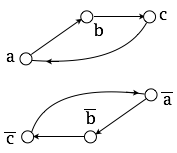
\includegraphics[width=0.25\textwidth]{FiguresGraph/2SATyes.png}
\caption{The digraph $\g(\Phi_1)$ and its two strongly connected components.}
  % provide a truth assignment for $\Phi_1$: $t(x_1) =  \mbox{\sc false}$; $t(x_2) = \mbox{\sc false}$; $t(x_3) = \mbox{\sc   true}$.}
\label{2SATyes}
\end{center}
\end{figure}
The graph has the two strongly connected components illustrated in the figure.  One thereby observes two satisfying truth-value assignments $t$ for formula $\Phi_1$:

\smallskip

\hspace*{.2in} $t(a) = t(b) = t(c) = \mbox{\sc true}$

\smallskip

or symmetrically

\smallskip

\hspace*{.2in} $t(a) = t(b) = t(c) = \mbox{\sc false}$.

\item
Fig.~\ref{2SATno} illustrates $\g(\Phi_2)$ for the formula
\[ \Phi_2 \ = \ (a \vee \bar{b}) \ \wedge \ (b \vee \bar{c}) \ \wedge \ (c \vee \bar{a})
 \ \wedge \ (a \vee c) \ \wedge \ (\bar{a} \vee \bar{c})
\]
\begin{figure}[htb]
\begin{center}
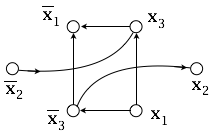
\includegraphics[width=0.25\textwidth]{FiguresGraph/2SATno.png}
\caption{The digraph $\g(\Phi_2)$}. 
% Because the graph  contains  a path from vertex $a$ to vertex $\bar{a}$,  formula  $\Phi_2$ does not admit any satisfying truth-assignment.}
\label{2SATno}
\end{center}
\end{figure}

Because the graph is strongly connected and contains directed paths in both directions between vertex $a$ and vertex $\bar{a}$, Proposition~\ref{prop:2SAT} assures us that formula $\Phi_2$ does not admit any satisfying truth assignment.
\end{enumerate}

\medskip

\noindent Even without invoking formal algorithmic concepts, it is clear that the processes of

\smallskip

$\bullet$ constructing digraph $\g(\Phi)$ from formula $\Phi$;

\noindent and

$\bullet$ isolating and investigating the strongly connected components of $\g(\Phi)$

\smallskip

\noindent
can be accomplished in a number of computational steps that is polynomial in the size of $\Phi$.  


%%%%%%%%%%%%%%%%%%%%%%%%%%%%%%%%%%%%

\subsection{Matchings in Graphs}
\index{graph!matching}

{\it Matching} are fundamental to many situations that can be modeled using graphs.  A {\it matching} in an undirected graph $\g$ is a set of edges of $\g$ that have no vertices in common.  In many computational settings, matchings are, thus, a convenient formal mechanism for pairing a graph's vertices.  The broad range of activities which can be modeled using graph matching
include: pairing competitors for a tennis tournament; helping a person select a potential spouse (which even in the vernacular is often termed ``matchmaking''); determining (near-)optimal layouts for a keyboard in language X (based on the relative ``affinities'' of various pairs of letters for one another in X); selecting persons to command the police stations in city Y (based on the
perceived ``match'' between a candidate's qualifications and the needs of specific stations).  Even this small sampler makes it clear that there are many significant variations on this formal theme.  This section is devoted to describing, and briefly discussing, a few of the most commonly encountered versions of matching in graphs.

\bigskip

\noindent \fbox{
\begin{minipage}{0.95\textwidth}
Although the definitions of the various versions of matching are readily accessible to even the mathematical novice, much of the more sophisticated mathematical knowledge about matchings is beyond any beginning text.  The interested reader might consult a more advanced source, such as \cite{Berge73}, to get a feeling for what is known about this conceptually simple, yet rich, topic.
\end{minipage}
}
\bigskip

\noindent {\it Matchings in unweighted graphs}.
The most straightforward notion of matching involves an undirected graph $\g$ with unlabeled edges.  The optimization criterion most often invoked with this genre of matching is to find a matching that involves as many edges of $\g$ as possible.

\smallskip

\index{graph!maximal matching}
\index{graph!maximal matching!unweighted graph}

The target in this ``vanilla-flavored'' matching problem is often a matching that is {\em maximal},  in the sense that adding any further edge of $\g$ to the matching leaves one with a set of edges that is no longer a matching.

\smallskip

\index{graph!perfect matching}

Among maximal matchings in a graph $\g$, the ``ultimate treasure'' is a matching that is {\it perfect}, in the sense that every vertex of $\g$ belongs to some edge of the matching.

\begin{prop}
\label{thm:max-matching}
Maximal matchings exist for any graph $\g$.  One can find such a matching in a number of steps proportional to $|\n|$.
\end{prop}

\index{greedy algorithm} 

\begin{proof}
We leave to the reader the challenge of verifying that the following {\em greedy}\footnote{\label{foot:greedy}In the world of algorithmics, the term ``greedy'' describes any process that seeks local optimizations, with no consideration of how such a myopic strategy might limit future options.}~process satisfies the conditions of the Proposition.

\medskip

\noindent
{\it The Process:} \\
Begin by laying the vertices of $\g$ out, left to right, in any way.

\smallskip

\noindent
Repeat the following process until no vertices remain in the layout.

\smallskip

\noindent
Select the leftmost vertex, $u$, in the remaining layout of $\n$.
  \begin{itemize}
  \item
If we succeed in finding such a neighbor of $u$ (taken from left to right)). call it vertex $v$, then add edge $\{u,v\}$ to the matching we are building.  Then, remove both $u$ and $v$ from the layout.
  \item
If there is no neighbor $v$ of $u$, then remove vertex $u$ from the layout.
  \end{itemize}
Of course, the real challenge here is to find a data structure that allows an efficient search for a ``remaining'' neighbor-vertex $v$ at each step of the selection process.  \qed
\end{proof}

\medskip

In contrast to maximal matchings, there exist myriad simple graphs that do not admit any perfect matching.  Contemplating, for instance, matchings within any cycle with an odd number of vertices may prepare the reader for the challenge of verifying the following necessary condition for a graph to admit a perfect matching.

\begin{prop}
\label{thm:necessary-for-perfect-matching}
Let $\g$ be a graph that admits a perfect matching.  Then:
\begin{itemize}
\item
$\g$ has an even number of vertices.
\item
The cardinality of the (perfect) matching---i.e., the number of edges in the matching---is exactly
$\frac{1}{2}|\n|$.
\end{itemize}
\end{prop}

\bigskip

\index{graph!maximal matching}

\noindent {\it Matchings in weighted graphs}.
The other very popular genre of matching problem focuses on graphs each of whose edges, say, $\{u,v\}$, is weighted with a number that measure the ``affinity'' of  vertices $u$ and $v$ for each other.  The challenge is to find a matching that is {\em maximal} in the sense of having a cumulative sum of edge-weights that is not exceeded by any other matching's.

\smallskip

%\index{Kuhn, Harold W.}

We note in closing that, while edge-weightings often complicate computational processing of graphs, they need not render such computations practically infeasible.  For instance, the problem of discovering a perfect matching of minimal weight in an edge-weighted graph can be solved moderately efficiently---i.e., in a number of steps that is polynomial in the size of the graph.  (One algorithm that achieves this efficiency can be based on the colorfully named {\it Hungarian assignment method}; see the original source \cite{Kuhn55} or the encyclopedic algorithms text \cite{CLRS}.)


%%%%%%%%%%%%%%%%%%%%%%%%%%%%%%%%%

\section{Trees and Spanning Trees}
\label{sec:Trees}

\index{graph!trees} \index{trees} \index{forest (of trees)} \index{graph!cycle-free}

The special class of graphs called {\it trees} occupy a place of honor within both the mathematical field called {\it graph theory} and within the vernacular.  Trees are identified mathematically as graphs that contain no cycles (as subgraphs) or, equivalently, as graphs in which each pair of vertices is connected by a unique path: a tree is thus the embodiment of ``pure'' connectivity:  it provides the minimal interconnection structure (in number of edges) that provides paths that connect every pair of vertices; see Fig.~\ref{fig:tree}.
\begin{figure}[hbt]
\begin{center}
       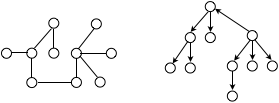
\includegraphics[scale=0.6]{FiguresGraph/tree}
       \caption{(Left) An undirected tree with 10 vertices.  (Right) A rooted directed out-tree.  (The root is not where you might expect it to be.)}
  \label{fig:tree}
\end{center}
\end{figure}
As one would expect from the vernacular, a set of trees is called a {\it forest}. 

\medskip

We have asserted implicitly that our two definitions of ``tree'' define the same class of graphs.  Of course, we do not accept this on faith---we must prove it.

\begin{prop}
\label{thm:2defns-trees}
The two definitions of ``tree'' are equivalent: they define the same class of graphs.  Stated more directly:

\smallskip

\noindent
The following assertions about a connected graph $\t$ are  logically equivalent. 
\begin{enumerate}
\item
The graph $\t$ is cycle-free.
\item
Each pair of distinct vertices of $\t$ is connected by precisely one path.
\end{enumerate}
\end{prop}

We leave the proof of Proposition~\ref{thm:2defns-trees} to the reader.

\bigskip

The following property of connected trees provides a valuable insight into myriad tree-related phenomena.  The property is a subtle  corollary of Proposition~\ref{thm:2defns-trees}.

\begin{prop}
\label{thm:edges-vs-nodes-tree}
An $n$-vertex connected tree $\t$ has precisely $n-1$ edges.
\end{prop}

We precede the proof by an essential lemma.

\begin{lemma}
\label{lem:vtx-deg-connected}
{\bf (a)}
Let $\g$ be a connected graph having $n \geq 2$ vertices.  Every vertex of $\g$ has degree $\geq 1$.

\smallskip

\noindent {\bf (b)}
Let $\t$ be a connected tree having $n \geq 1$ vertices.  At least one vertex of $\t$ has degree $1$.
\end{lemma}

\begin{proof}[Lemma~\ref{lem:vtx-deg-connected}]
{\bf (a)} A vertex of $\g$ that had degree $0$ would have no neighbors; hence, $\g$, having $n \geq 2$ vertices, would not be connected if it had such a vertex.

\smallskip

\noindent {\bf (b)}
By Proposition~\ref{thm:cycle-in-graph} every graph whose vertices all have degree $\geq 2$
contains a cycle.  Since $\t$, being a tree, is cycle-free, not every vertex of $\t$ can have degree $\geq 2$.  By part {\bf (a)}, then, at least one vertex of tree $\t$ has degree $1$.  \qed
\end{proof}

\begin{proof}[Proposition~\ref{thm:edges-vs-nodes-tree}]
We proceed by induction on $n$.

\smallskip

\noindent {\sf Base case}.
The case $n=2$ is obvious, because a single edge is both necessary and sufficient to connect two vertices.

\smallskip

\noindent {\sf Inductive hypothesis}.
Assume that the indicated tally is correct for all trees having no more than $k$ vertices.

\smallskip

\noindent {\sf Inductive extension}.
Consider, to extend the induction, any tree $\t$ on $k+1$ vertices.  

\smallskip

By Lemma~\ref{lem:vtx-deg-connected}, $\t$ must contain at least one vertex $v$ of degree $1$.  If we remove $v$ and its (single) incident edge, we now have a tree $\t'$ on $k$ vertices.
By induction, $\t'$ has $k-1$ edges.  When we reattach vertex $v$ to $\t'$, we restore $\t$ to its original state.  Because this restorations adds one vertex and one edge to $\t'$, we see that $\t$ has $k+1$ vertices and $k$ edges.

\smallskip

This extends the induction, hence completes the proof.  \qed
\end{proof}

\bigskip

\index{trees!parent vertex}
\index{trees!child vertex}
\index{trees!ancestor vertex}
\index{trees!descendant vertex}
\index{trees!root (vertex)} \index{root (of a directed tree)} 
\index{trees!leaf (vertex)}\index{leaf (of a directed tree)}

Just as with graphs, there is a {\em directed} version of trees, which is formed by replacing
the (nonoriented) edges of an undirected tree by (oriented) arcs; see Fig.~\ref{fig:tree}(right).  Within a directed tree $\t$, one often says that an arc goes {\em from} a {\it parent vertex} {\em to} a {\it child vertex}.  Extending this anthropomorphic metaphor, one often talks about the {\it ancestor(s)}  and {\it descendant(s)} of a tree-vertex.  We single out two special classes of vertices: A {\it root (vertex)} of $\t$ is defined by having no entering arcs, i.e., by having indegree $0$; a {\it leaf (vertex)} of $\t$ is defined by having no exiting arcs, i.e., by having outdegree $0$.

\bigskip

\noindent \fbox{
\begin{minipage}{0.96\textwidth}
Note that the directed tree in Fig.~\ref{fig:tree}(right) is rooted, but we have not drawn the tree in the usual way, with the root either above or below all other vertices.  This was a purposeful decision, so that the reader would note that root-hood is a property of graph structure, not of drawing.
\end{minipage}
}

\bigskip

The reader is certainly familiar with the use of rooted directed trees to represent family trees and corporate hierarchies, as described in the following examples.

\bigskip

\index{family tree}

\noindent \fbox{
\begin{minipage}{0.96\textwidth}
Sociologically, the historical {\it atomic family tree} has two roots, representing the matriarch and patriarch of the family.  The entirety of the tree represents a single family generationally, before any children form their own families.  All child-vertices in this genre of tree are the roots of singly-rooted subtrees of the entire family tree.  The leaves of the tree are the childless descendants of the roots.  Note that, while we are using anthropomorphic language here, we could be discussing other genres of ``family'', as, e.g., many types of biological taxonomies.
\end{minipage}
}

\bigskip

\index{generation of a vertex in a singly-rooted directed tree}

Among rooted directed trees, an important subclass comprises those that have a {\em single root} which has a directed path to every other vertex.  The length of each such directed path is often used to label the {\it generation} of the vertex at the end of the path: root, child, grandchild,
great-grandchild, etc.  Every vertex of the tree is the root of a singly-rooted directed subtree of the entire tree.  All subtrees that are rooted at vertices of the same generation are mutually disjoint.

\bigskip

\index{trees!singly-rooted!hierarchy} \index{hierarchy}

\noindent \fbox{
\begin{minipage}{0.96\textwidth}
A singly-rooted tree represents a {\it hierarchy}.  Given two directed subtrees within a hierarchy, either the root of one of the subtrees is a descendant of the root of the other, or the two subtrees
are mutually disjoint.
\end{minipage}
}

\bigskip


\ignore{****************
More formally: {\em rooted trees} are a class of {\em acyclic}
digraphs.  Paths in trees which start at the root are often called
{\em branches}.  The {\em acyclicity} of a tree $\t$ means that for
any branch of $\t$ of the form (\ref{eq:di-path}), we cannot have $u_1
= u_n$, for this would create a cycle.  Each singly-rooted tree $\t$
has a designated {\em root vertex} \index{trees!root vertex} $u_n \in
\n_{\ft}$ that resides at the end of a branch (\ref{eq:di-path}) that
starts at $r_{\ft}$ (so $u_1 = r_{\ft}$) is said to reside at {\em
  depth} $n-1$ in $\t$; by convention, $r_{\ft}$ is said to reside at
depth $0$.  \index{depth of a vertex in a singly-rooted tree} $\t$'s
root $r_{\ft}$ has some number (possibly $0$) of arcs that go from
$r_{\ft}$ to its {\em children,} each of which thus resides at depth
$1$ in $\t$; in turn, each child has some number of arcs (possibly
$0$) to its children, and so on.  For each arc $(u \rightarrow v) \in
A_{\ft}$, we call $u$ a {\it parent} \index{trees!parent vertex} of $v$,
and $v$ a {\it child} \index{trees!child vertex} of $u$, in $\t$;
clearly, the depth of each child is one greater than the depth of its
parent.  Every vertex of $\t$ except for $r_{\ft}$ has precisely one
parent; $r_{\ft}$ has no parents.  A childless vertex of a tree is a
{\em leaf}, \index{trees!leaf vertex} i.e., a vertex of degree $1$.  The
transitive extensions of the parent and child relations are,
respectively, the {\em ancestor} \index{trees!ancestor vertex} and {\em
  descendant} \index{trees!descendant vertex} relations.  The {\em
  degree} \index{degree (of a vertex in a tree)} of a vertex $v$ in a tree
is the number of children that the vertex has, call it $c_v$.  If every
non-leaf vertex in a tree has the same degree $c$, then we call $c$ the
{\em degree of the tree}.  \index{degree of a tree}

It is sometimes useful to have a symbolic notation for the ancestor
and descendant relations.  To this end, we write $(u \Rightarrow v)$
\index{$\Rightarrow$: ancestor/descendant in a rooted tree} to
indicate that vertex $u$ is an {\it ancestor} of vertex $v$, or
equivalently, that vertex $v$ is a {\it descendant} of vertex $u$.  
{\Denis Do we use the notation later? If not, we should remove it...}
If we
decide that we are not interested in {\em really distant} descendants
of the root of a tree $\t$, then we can {\em truncate} \index{truncated}
$\t$ at a desired depth $d$ by removing all vertices whose depths exceed
$d$.  We thereby obtain the {\em depth-$d$ prefix} of $\t$.

Figure \ref{fig.graph-samples} depicts an arc-labeled rooted tree $\t$
whose arc labels come from the alphabet $\{a,b\}$.  $\t$'s arc-induced
relationships are listed in Table~\ref{tab.graph-samples}.
\begin{figure}[htb]
\centerline{\epsfig{figure=graph.sample.eps,height=4truecm}}
\caption{An arc-labeled rooted tree $\t$ whose arc labels come from
  the alphabet $\{a,b\}$.  (Arc labels have no meaning; they are just
  for illustration.)
\label{fig.graph-samples}}
\end{figure}
\begin{table}[htb]
{\small
\begin{center}
\fbox{
\begin{tabular}{c||c|c|c|c}
\multicolumn{5}{c}{The arc-labeled rooted tree $\t$ of
  Figure \ref{fig.graph-samples}} \\
\hline
Vertex            & Children & Parent & Descendants & Ancestors \\
\hline
\hline
$r_{\ft} = u_0$ 
& $u_1$
& none & 
$u_1, u_2, \ldots, u_k, v_1, v_2, \ldots, v_k,
w_1, w_2, \ldots, w_k$
& none \\
\hline
$u_1$
& $u_2, v_1$
& $u_0$ & 
$u_2, \ldots, u_k, v_1, v_2, \ldots, v_k, w_1, w_2, \ldots, w_k$
& $u_0$ \\
\hline
$u_2$
& $u_3, v_2$
& $u_1$ & 
$u_3, \ldots, u_k, v_2, \ldots, v_k, w_2, \ldots, w_k$
& $u_0$ \\
\hline
 $\vdots$ & $\vdots$ & $\vdots$ &  $\vdots$ &  $\vdots$ \\
\hline
$u_k$
& $v_k$ 
& $u_{k-1}$ & 
$v_k, w_k$
& $u_0, u_1, \ldots, u_{k-1}$ \\
\hline
$v_1$
& $w_1$ 
& $u_1$ & 
$w_1$
& $u_0, u_1$ \\
\hline
$v_2$
& $w_2$
& $u_2$ & 
$w_2$
& $u_0, u_1, u_2$ \\
\hline
 $\vdots$ & $\vdots$ & $\vdots$ &  $\vdots$ &  $\vdots$ \\
\hline
$v_k$
& $w_k$
& $u_k$ & 
$w_k$
& $u_0, u_1, \ldots, u_k$ \\
\hline
$w_1$
& none
& $v_1$ & 
none
& $u_0, u_1, v_1$ \\
\hline
$w_2$
& none &
$v_2$ & 
none
& $u_0, u_1, u_2, v_2$ \\
\hline
$w_k$
& none
& $v_k$ & 
none
& $u_0, u_1, \ldots, u_k, v_k$
\end{tabular}
}
\end{center}
}
\caption{A tabular description of the rooted tree $\t$ of
  Figure \ref{fig.graph-samples}.  \label{tab.graph-samples}}
\end{table}
*********************}

\index{graph!spanning tree} \index{spanning tree} \index{tree!spanning tree}

\noindent {\it Spanning trees}.
One of the major uses of trees and forests is as a way of succinctly ``summarizing'' the connectivity structure inherent in an undirected graph.  This role is inherent in the notion of a {\it spanning tree} of a connected graph $\g$.  A spanning tree of $\g$ is a tree $\t(\g)$ whose vertex-set is identical to $\g$'s:
\[ \n_{\ft(\fg)} \ = \ \n_{\fg} \]
and all of whose edges are edges of $\g$:
\[ \e_{\ft(\fg)} \ \subseteq \ \e_{\fg}. \]
Not surprisingly, a connected graph $\g$  typically has {\em many} spanning trees.  All such trees share $\g$'s vertex-set, but they may choose quite different sets of edges.

\ignore{*************
For a graph $\g$ that is not connected, we replace the notion of
spanning tree of $\g$ with the analogous notion of a {\it spanning
  forest} \index{graph!spanning forest} \index{spanning forest} of
$\g$.  We shall typically discuss only spanning trees in this section,
leaving the reader to extrapolate the discussion to include spanning
forests of unconnected graphs.
****************}

\smallskip

\index{graph!spanning tree!edge-weighted} \index{graph!minimum-weight spanning tree}
\index{minimum-weight spanning tree} 

Within applications, as a spanning tree ``summarizes'' the connectivity structure of a graph, it does the same for any entities that the graph models, such as a map, the layout of a museum, etc.  This modeling role makes spanning trees invaluable as the basis for algorithms that involve connectivity-related notions.  To encompass an even greater range of such notions, we often {\it weight} the edges of spanning trees, in order to model a ``cost'' of incorporating that edge into the tree.  The types of computational problem modeled via edge-weighted spanning trees include: the optimal placement of firehouses, or hospitals, in a town and the optimal deployment of security mechanisms in an art museum.  Reflecting problems wherein edge-weights measure transit costs, it is a classical computational problem to seek a {\em minimum-weight spanning tree} (usually abbreviated in the vernacular to {\em minimum spanning tree}).  Happily, this classical optimization problem can be solved within a number of steps that is linear in the number of edges of $\g$ \cite{CLRS}.


%%%%%%%%%%%%%%%%%%%%%%%%%%%%%%%%%%%

\section{Computationally Significant ``Named'' Graphs}
\label{sec:graphs-important-families}

The area of mathematics called graph theory is an important source of formal aids for designing, analyzing, utilizing, modeling, and verifying systems that are used for computation and/or communication.  Of course, such systems are designed by humans.  Among the manifold consequences of this fact is the observation that the (families of) graphs that are among the most commonly used to model systems tend to be rather uniform in structure, in a variety of ways: Such graphs, when drawn, often exhibit a lot of structural regularity.  We single out one particularly popular form of structural regularity to watch for as we prepare to describe five families of graphs that have proven so significant as models of variety of computational and communicational processes that they are usually referred to just by their given names.  (We noted a similar phenomenon early in Chapter~\ref{ch:numerals}, as we discussed numbers such as $e$ and $\pi$ and Avogadro's number.)  The notion of regularity that we single out is so popular that it is familiarly known as just {\it ``regularity",} even though its complete name is
{\it ``degree regularity"}.
\begin{itemize}
\item
{\em Undirected version}.
An undirected graph $\g$ is {\it (degree-)regular} if all of its vertices have the same degree.
\item
{\em Directed version}.
A directed graph $\g$ is {\it (degree-)in-regular} if all of its vertices have the same in-degree.  $\g$ is {\it (degree-)out-regular} if all of its vertices have the same out-degree.
\end{itemize}

\index{graph!directed!in-regular} \index{graph!directed!out-regular} \index{graph!regular}

\medskip

We now describe five families of regular graphs that have proven useful for understanding and implementing both computation and communication over the entire digital era, and we expose some basic properties of each.  Each of these graphs is available in both a directed and an undirected version, although, as we note, for each, one of these versions is more commonly encountered.  We have selected these specific graphs for rather different reasons.
\begin{itemize}
\item
The first two graphs, the {\it cycle-graph} of Section~\ref{sec:cycle} and the {\it complete graph} (or, {\it clique}) of Section~\ref{sec:clique} were selected for representing, respectively, the lowest-degree and highest-degree graphs that share two properties:
\begin{enumerate}
\item
Every vertex of each graph is accessible from every other vertex.
\item
All vertices of each graph ``look alike'' to someone traversing the graph.

\smallskip

To elaborate: If someone places you on a vertex of either graph, there is no way that you can determine the identity of that vertex.

\smallskip

\index{anonymity}

This is an important feature to ponder, because it is a simple instance of the {\it anonymity} problem that plagues many modern distributed computing environments:  {\it How does one orchestrate cooperative activities when all agents are ``indistinguishable''?}
\end{enumerate}
\item
The remaining graphs, the {\it mesh and torus networks}\footnote{These two structures, though distinct, are usually discussed together because they share so many important properties.}~of~\ref{sec:mesh}, the {\it hypercube network} of Section~\ref{sec:hypercube}, and the {\it de Bruijn network} of Section~\ref{sec:deBruijn}, were selected for their importance within the world of parallel and distributed computing---as abstract platforms for developing efficient computational and communicational processes, and as abstract versions of the networks that underlie parallel architectures by interconnecting its processors.

\smallskip

The hypercube network and the de Bruijn network are known also as indispensable aids in constructing codes that are used in activities as varied as cryptology and the testing of electronic circuits.
\end{itemize}
Throughout this section, each parameter $n$ that identifies an instance from our graph families ranges over either $\N$ or $\N^+$; we shall always indicate which.

\subsection{The {\it Cycle-graph} $\cc_n$}
\label{sec:cycle}

\index{cycle graph} \index{cycle network}  \index{cycle graph!vertex-degree}
\index{cycle graph!predecessor vertex}
\index{cycle graph!successor vertex} \index{cycle graph!diameter}

For each positive integer $n \in \N^+$, both the {\it undirected order-$n$ cycle-graph} $\cc_n$ and the {\it directed order-$n$ cycle-graph} $\widehat{\cc}_n$  have {\it vertex-set}
\[ \n_{{\cal C}_n} \ = \ \n_{\widehat{{\cal C}}_n} \ = \ \{ 0, \ 1, \ \ldots, \ n-1\}. \]
\begin{itemize}
\item
$\cc_n$ has $n$ edges; its {\it edge-set} is
\[ \e_{{\cal C}_n} \ = \ \big\{ \{i, \ i+1 \bmod n\} \ \ | \ \ i \in \{0, \ 1, \ \ldots, \ n-1\} \big\}.  \]
Fig.~\ref{fig:cycle} depicts the $8$-vertex cycle $\cc_8$.
  \begin{itemize}
  \item
$\cc_n$ is degree-regular: each vertex has degree $2$.

\smallskip

Specifically, each vertex $i$ of $\cc_n$ has its {\it predecessor} $i-1 \bmod n$ and its {\it successor} $i+1 \bmod n$.

  \item 
$\cc_n$ has diameter $\lfloor n/2 \rfloor$.

\smallskip

Direct calculation shows that $\cc_n$'s diameter is no larger than $\lfloor n/2 \rfloor$.  The fact that this is, in fact, the graph's diameter is witnessed by the distance between each vertex $k \in \n_{{\cal C}_n}$ and its antipodal vertex $k + \lfloor n/2 \rfloor \bmod n$.
  \end{itemize}

\item
$\widehat{\cc}_n$ has {\it arc-set}
\[ \a_{\widehat{{\cal C}}_n} \ = \ 
\big\{ (i \rightarrow i+1 \bmod n) \ \ | \ \ i \in \{0, \ 1, \ \ldots, \ n-1\} \big\}
\]
  \begin{itemize}
  \item 
$\widehat{\cc}_n$ is a regular directed network: each vertex has in-degree and out-degree $2$.
  \item
$\widehat{\cc}_n$ has (directed) diameter $n-1$.

\smallskip

Of course, $n-1$ is an upper bound on the diameter of any $n$-vertex digraph.  The fact that this is exactly $\widehat{\cc}_n$'s diameter is witnessed by the directed distance from each vertex $k$ of $\widehat{\cc}_n$ to its predecessor vertex $k-1 \bmod n$.
  \end{itemize}
\end{itemize}
\index{cycle graph!directed vertex-degree}

\begin{figure}[hbt]
\begin{center}
       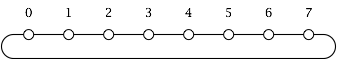
\includegraphics[scale=0.6]{FiguresGraph/cycle}
       \caption{The $8$-vertex cycle $\cc_8$.}
  \label{fig:cycle}
\end{center}
\end{figure}

\subsection{The {\it Complete graph}, or, {\it Clique} $\k_n$}
\label{sec:clique}
\index{complete graph} \index{clique} 
\index{complete graph!vertex-degrees} \index{clique!vertex-degrees}
\index{complete graph!diameter}

For each positive integer $n \in \N^+$, we denote by $\k_n$ the {\em undirected} order-$n$ {\it complete-graph} (or, {\it clique}), and by $\widehat{\k}_n$ the {\em directed} order-$n$ {\it complete-graph} (or, {\it clique}).  Both $\k_n$ and $\widehat{\k}_n$ have {\it vertex-set}
\[ \n_{{\cal K}_n} \ = \ \n_{\widehat{{\cal K}}_n} \ = \ \{ 0, \ 1, \ \ldots, \ n-1\}. \]
\begin{itemize}
\item
$\k_n$ has $\displaystyle {n \choose 2}$ edges; its {\it edge-set} is
\[ \e_{{\cal K}_n} \ = \ \big\{ \{i, \ j\} \ \ | \ \ i,j \in \{0, \ 1, \ \ldots, \ n-1\}, \ i \neq j \big\}. \]
  \begin{itemize}
  \item 
$\k_n$ is a regular network: each vertex has degree $n-1$; every vertex $i \in \n_{\fk_n}$ is a neighbor of every other vertex.

   \item \index{complete graph!diameter}
$\k_n$ has diameter $1$.

\smallskip

$\k_n$'s diameter is a direct consequence of its vertex-degrees, and vice versa.
  \end{itemize}

\item
$\widehat{\k}_n$ has $(n-1)n$ arcs; its {\it arc-set} is
\[ \a_{\widehat{{\cal K}}_n} \ = \ 
\big\{ (i \rightarrow j) \ \ | \ \ i,j \in \{0, \ 1, \ \ldots, \ n-1\} \big\}, \ i \neq j \]
  \begin{itemize}
  \item
$\widehat{\k}_n$ is a regular directed network: each vertex has in-degree and out-degree $n-1$.
  \item
$\widehat{\k}_n$ has (directed) diameter $1$.

\smallskip

$\widehat{\k}_n$'s diameter and its (in- and out-) vertex-degrees determine one another.
  \end{itemize}
\end{itemize}

\ignore{********
{\Denis good opportunity for an exercice here: a tournoiment 
is a directed version of a complete graph (any orientation of the edges).
The proof that it is hamiltonian is nice, If you agree I can add it in the exercices...}
***********}

\medskip

Hearkening back to our discussion of matchings in (unweighted) graphs: The structure of the set of perfect matchings in general graphs is decidely nontrivial.  For clique-graphs, though, the structure is much easier to discuss.

\begin{prop}
\label{thm:perfect-matchings-clique}
The number of perfect matchings admitted by the clique-graph $\k_n$ is either $0$---if $n$ is odd---or exponential in $n$---if $n$ is even.
\end{prop}

\begin{proof}
The assertion about cliques with odd numbers of vertices is immediate
(see Proposition~\ref{thm:necessary-for-perfect-matching}): one vertex can never been paired.

\smallskip

We verify the assertion about cliques of the form $\k_{2k}$ by induction on $k$.  To this end, let $M_n$ denote the number of perfect matchings that $\k_n$ admits.

\smallskip

We are going to fashion this proof to reflect the way that a mathematician would reason, rather than presenting the highly structured form of induction that we have been using until now.  After all, we are already in Chapter 12!

\medskip

\noindent 
The base case $k=1$ is immediate:  Because $\k_{2}$ consists of a single edge, it admits precisely one perfect matching; i.e., $M_1 = 1$.
%(see Figure~\ref{perfectMatching1}): 

\smallskip

To garner intuition, we also explicitly solve the case $k=2$, which is illustrated in Fig.~\ref{fig:AllPerfectMatchings}.
\begin{figure}[hbt]
\begin{center}
       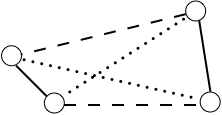
\includegraphics[scale=0.55]{FiguresGraph/perfectmatchingAll}
       \caption{$\k_4$ (left) and its three different perfect matchings (right):  The matchings' edges are drawn, respectively, with bold lines, dashed lines, and dotted lines.}
  \label{fig:AllPerfectMatchings}
\end{center}
\end{figure}
As the figure illustrates, $\k_4 = \k_{2 \cdot 2}$ can be viewed as a $4$-cycle (drawn with bold and dashed lines), augmented by two ``cross-edges'' (drawn with dotted lines).  Easily, then, $\k_4$ admits $3$ different perfect matchings, which can be identified (and specified) by the edge that contains the northwesterly vertex---call it $v$---in the figure.  Vertex $v$ has the choice of three vertices to ``boldly'' match with. (In the figure, $v$ has chosen the southwesterly vertex as its ``bold'' match.)  Once $v$ has chosen its match, there is only one viable choice for the second edge in the matching.  Thus, $M_2=3$.

\medskip

We jump now to the case of any arbitrary $k > 2$.  We remark that there are precisely $2k-1$ vertices of $\k_{2k}$ that vertex $1$ can ``choose'' as its mate in a perfect matching.  Once we match vertex $1$ to its mate, we confront an independent instance of the perfect-matching-counting problem with parameter $k-1$---i.e., the problem of counting the number of perfect matchings in $\k_{n-2} = \k_{2k-2}$.  We thereby note that as $k$ grows, the quantity $M_k$ obeys the following recurrence:
\[ M_k \ = \ (2k-1) \times M_{k-1} \]
In other words:

\smallskip

\hspace*{.25in}{\em $M_k$ is the product of the first $k$ odd numbers.}
%$N_1=1$, $N_2=3$, $N_3=3 \times 5=15$, $N_4=3 \times 5 \times 7=115$, etc..

\smallskip

\noindent
To gauge the growth rate of $M_k$, we concentrate on cases $k > 2$ and ignore the $\lfloor k/2 \rfloor$ smallest odd numbers.  We then replace each of the remaining odd numbers by its smallest possible value.  We thereby find that
\[
M_k \ \ =    \ \ \prod_{i=1}^k \ (2i-1)
    \ \ \geq \ \ \prod_{\lceil k/2 \rceil}^k \ (2i-1)
    \ \ \geq \ \ \left( 2 \lceil k/2 \rceil -1 \right)^{k/2}
    \ \ >    \ \ k^{k/2}
\]
In summary, $M_k$ grows exponentially with the parameter $k$, as claimed.  \qed
\end{proof}

\bigskip

The two families of graphs we have discussed thus far---cycles and cliques---are recommended by their structural simplicity:  They epitomize, respectively, the most sparse way (the cycle) and the most dense way (the clique) to completely interconnect $n$ vertices.  The remainder of this section is devoted to three families of graphs which have been found to be very useful in computational and communicational scenarios.  These graphs' structures are simple enough to be amenable to rigorous reasoning, while being rich enough to support a broad range of procedures that have been shown to afford one access to craft algorithms that exploit the potential efficiencies---in computation and communication---that one can achieve using modern technologies.

\subsection{Sibling Networks: the {\it M}esh ($\m_{m,n}$); the {\it Torus} ($\widetilde{\m}_{m,n}$)}
\label{sec:mesh}
\index{mesh and torus networks}

For positive integers $m, n \in \N^+$, both the $m \times n$ {\it mesh (network)} $\m_{m,n}$ and the $m \times n$ {\it toroidal network} (or, {\it torus}) $\widetilde{\m}_{m,n}$ have {\it vertex-set}
\begin{eqnarray*}
\n_{\fm_{m,n}} \ = \ \n_{\widetilde{\fm}_{m,n}}
  & = & 
\{1, \ 2, \ldots, \ m\} \ \times \ \{1, \ 2, \ldots, \ n\} \\
  & = & 
\big\{ \langle i, \ j \rangle \ \ | \ \ 
\big[ i \in \{1, \ 2, \ldots, \ m\} \big], \ \ \big[ j \in \{1, \ 2, \ldots, \ n\} \big]
\big\}
\end{eqnarray*}

\begin{itemize}
\item
$\m_{m,n}$ has $(m-1)n \ + \ (n-1)m$ edges; its {\it edge-set} is
\begin{eqnarray*}
\e_{\fm_{m,n}} & = & 
\big\{
\{ \{ i, j \}, \ \{ i+1, j \} \ \ | \ \
1 \leq i < m, \ \ 1 \leq j \leq n \} \\
  &  & \hspace*{.1in} \cup \ \
\{ \{ i, j \}, \ \{ i, j+1 \} \ \ | \ \ 1 \leq i \leq m, \ \ 1 \leq j < n \}
\big\}
\end{eqnarray*}

\index{row of a mesh graph}\index{mesh graph!row}
\index{column of a mesh graph}\index{mesh graph!column}

\begin{itemize}
\item
The subgraph of $\m_{m,n}$ defined by the vertex-set
\[ \{ \langle i, \ j \rangle  \ \ | \ \ \left[i \in \{1, 2, \ldots, m\}\right], \ \ \left[1 \leq j < n\right]\} \]
and all edges both of whose endpoints belong to that set is the $i$th {\it row} of $\m_{m,n}$.  Dually, the subgraph of $\m_{m,n}$ defined by the vertex-set
\[ \{ \langle i, \ j \rangle  \ \ | \ \ \left[j \in \{1, 2, \ldots, n\}\right], \ \ \left[1 \leq i < m\right] \} \]
and all edges both of whose endpoints belong to that set is the $j$th {\it column} of $\m_{m,n}$.

\ignore{*********************
  \begin{itemize}
     \item
Vertices $\langle 1, \ 1 \rangle$, $\langle 1, \ n \rangle$, $\langle m,
\ 1 \rangle$, and $\langle m, \ n \rangle$ are the {\it corner vertices}
(or, just {\it corners}) of $\m_{m,n}$.
\index{corner (vertex) of a mesh graph}
\index{mesh graph!corner (vertex)}
     \item
The path-graph consisting of the vertex-set
\[ \{ \langle 1, \ 1 \rangle, \ \langle 1, \ 2 \rangle, \ldots, \
\langle 1, \ n \rangle \}
\]
together with all edges of $\m_{m,n}$ both of whose endpoints belong
to this set, is the {\it top edge} of $\m_{m,n}$.
\index{top edge of a mesh graph}
\index{mesh graph!top edge}

The other edges of $\m_n$ are defined analogously:

\smallskip

The {\it bottom edge} of $\m_{m,n}$ is the path-graph built upon the
vertex-set
\[ \{ \langle m, \ 1 \rangle, \ \langle m, \ 2 \rangle, \ldots, \
\langle m, \ n \rangle \}
\]
\index{bottom edge of a mesh graph}
\index{mesh graph!bottom edge}

The {\it left edge} of $\m_{m,n}$ is the path-graph built upon the
vertex-set
\[ \{ \langle 1, \ 1 \rangle, \ \langle 2, \ 1 \rangle, \ldots, \
\langle m, \ 1 \rangle \}
\]
\index{left edge of a mesh graph}
\index{mesh graph!left edge}

The {\it right edge} of $\m_{m,n}$ is the path-graph built upon the
vertex-set
\[ \{ \langle 1, \ n \rangle, \ \langle 2, \ n \rangle, \ldots, \
\langle m, \ n \rangle \}
\]
\index{left edge of a mesh graph}
\index{mesh graph!right edge}
     \end{itemize}
**********************}

  \item 
$\m_{m,n}$ is {\em not} a regular graph.  Its four corner vertices each has degree $2$; its non-corner extreme edge vertices each has degree $3$; its {\em internal vertices} each has degree $4$.

\index{mesh graph!vertex-degree} \index{internal vertex of a mesh graph}
\index{mesh graph!internal vertex}

  \item \index{mesh graph!undirected diameter}
The diameter of $\m_{m,n}$ is $m+n-2$, as witnessed by the distance between vertices $\langle 1, \ 1 \rangle$ and $\langle m, \ n \rangle$.
  \end{itemize}
 \index{mesh graph!undirected diameter}

\item
$\widetilde{\m}_{m,n}$ has $2mn$ arcs; its {\it arc-set} is
\begin{eqnarray*}
\a_{\widetilde{\m}_{m,n}} & = &
\big\{
\{ (\langle i, \ j \rangle \rightarrow \langle i+1 \bmod m, \ j \rangle) \ \ | \ \ 1 \leq i \leq m, \ \ 1 \leq j \leq n \} \\
  &  & \hspace*{.1in} \cup \ \
\{ (\langle i, \ j \rangle \rightarrow \langle i, \ j+1 \bmod n \rangle) \ \ | \ \ 1 \leq i \leq m, \ \ 1 \leq j \leq n \}
\big \}
\end{eqnarray*}

\ignore{***********
  \begin{itemize}
  \item
The subgraph of $\widetilde{\m}_{m,n}$ defined by the vertex-set
\[ \{ \langle i, \ j \rangle  \ \ | \ \ \left[i \in \{1, 2, \ldots,
  m\}\right], \ \ \left[1 \leq j \leq n\right]\}
\]
and all edges both of whose endpoints belong to that set is called the
$i$th {\it row} of $\widetilde{\m}_{m,n}$
\index{torus graph!row}
Dually, the subgraph of$\widetilde{\m}_{m,n}$ defined by the vertex-set
\[ \{ \langle i, \ j \rangle  \ \ | \ \ \left[j \in \{1, 2, \ldots,
  n\}\right], \ \ \left[1 \leq i \leq m\right] \}
\]
and all edges both of whose endpoints belong to that set is called the
$j$th {\it column} of $\widetilde{\m}_{m,n}$.
\index{torus graph!column}
**********}
\begin{itemize}
  \item
$\widetilde{\m}_{m,n}$ is a regular network; each vertex has degree $4$.  Despite the fact that $\widetilde{\m}_{m,n}$ is an {\em undirected} graph, its edges are commonly referred to via an  anthropomorphic directional labeling, as ``up, down, left, and right''  or as ``north, south, west, and east''.
  \item
$\widetilde{\m}_{m,n}$'s diameter is $\lfloor m/2 \rfloor \ + \ \lfloor n/2 \rfloor$.  This can be verified by analogy to the diameter of the cycle-graph $\cc_n$.  \index{mesh graph!directed diameter}
\end{itemize}
\end{itemize}

\begin{figure}[hbt]
\begin{center}
       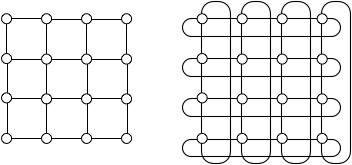
\includegraphics[scale=0.6]{FiguresGraph/meshtorus}
       \caption{$\m_{4,4}$ (left) and $\widetilde{\m}_{4,4}$ (right).}
  \label{fig:torus}
\end{center}
\end{figure}

\subsection{The (Boolean) {\it Hypercube} $\q_n$}
\label{sec:hypercube}
\index{boolean hypercube}
\index{hypercube}

The graphs we focus on in this section have had a major impact on the world of coding, especially in regard to codes that are {\em error correcting} \cite{PetersonW81}, and on the world of computing, especially in regard to parallel and distributed computing
\cite{JohnssonH1989, SaadS89, Schwartz80}.  The cited sources give a range of perspectives on the importance of {\it hypercube networks.}

\index{order-$n$ boolean hypercube}
The {\it order-$n$ boolean hypercube}, traditionally denoted $\q_n$, is the $2^n$-vertex graph defined via one of the following (equivalent) definitions.
\begin{itemize}
\item
{\it The recursive definition}. 
\index{order-$n$ boolean hypercube!recursive definition}
  \begin{itemize}
  \item
The order-$0$ boolean hypercube, $\q_0$, has a single vertex, and no edges.
  \item
The order-$(k+1)$ boolean hypercube, $\q_{k+1}$, is obtained by taking two copies of $\q_k$, call them $\q_k^{(1)}$ and $\q_k^{(2)}$, and creating an edge that connects each vertex of $\q_k^{(1)}$ with the corresponding vertex of $\q_k^{(2)}$.
  \end{itemize}
For illustration:
  \begin{itemize}
  \item
$\q_1$ consists of two vertices connected by a single edge.
  \item
$\q_2$ can be viewed as a ``square'', or equivalently, a copy of the $4$-cycle $\cc_4$.
  \item
$\q_3$ can be viewed as a ``cube'', i.e., as two copies of $\cc_4$ with edges connecting corresponding vertices: Each of the following pairs of vertices are connected by an edge:

\smallskip

\hspace*{.25in}\begin{tabular}{l}
the upper right corner-vertices \\
the upper left corner-vertices \\
the lower right corner-vertices \\
the lower left corner-vertices
\end{tabular}
  \end{itemize}

\item
{\it The direct definition}.
For each $n \in \N$, the vertices of the order-$n$ boolean hypercube,
$\q_n$, are all length-$n$ binary strings.  For illustration:
\index{order-$n$ boolean hypercube!direct definition}

\smallskip

\hspace*{.25in}\begin{tabular}{l}
$\n_{{\fq}_0}
  \ = \ 
\{ \varepsilon \}$, \ \ \ the length-$0$ {\em null string} \\ 
$\n_{{\fq}_1}
  \ = \ \{ 0, \ 1 \}$ \\
$\n_{{\fq}_2}
  \ = \ \{ 00, \ 01, \ 10, \ 11 \}$ \\
$\n_{{\fq}_3}
  \ = \ \{ 000, \ 001, \ 010, \ 011, \ 100, \ 101, \ 110, \ 111 \}$
\end{tabular}

\smallskip

The iteration-based construction of big hypercubes from the next smaller ones is illustrated in Fig.~\ref{fig:hypercube}.
\begin{figure}[hbt]
\begin{center}
       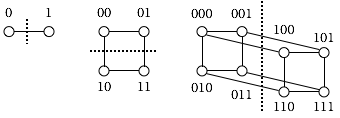
\includegraphics[scale=0.6]{FiguresGraph/hypercube}
\caption{The iteration-based construction of order-$n$ hypercubes:  (1) Take two copies of the order-$(n-1)$ hypercube.  (2) Prepend a $0$ to the vertex-labels of the first copy and a $1$ to the vertex-labels of the second copy.}
  \label{fig:hypercube}
\end{center}
\end{figure}

\smallskip

Easily, each $\q_n$ has $2^n$ vertices, for this is the number of length-$n$ binary strings.

\medskip

For each value of $n$, each edge of $\q_n$ connects two vertex-strings that differ in precisely one bit-position.  This means that $\q_n$ has $n 2^{n-1}$ edges: To wit, each of its $2^n$ vertices has $n$ neighbors, so the quantity $n 2^n$ counts each of $\q_n$'s edges twice---one for each endpoint.  For illustration:
\begin{eqnarray*}
\e_{{\fq}_1}
  & = &
\big\{ \{ 0, \ 1 \} \big\} \\
\e_{{\fq}_2}
  & = & \big\{
\{ 00, \ 01 \}, \ \{ 00, \ 10\}, \
\{ 01, \ 11 \}, \ \{ 10, \ 11\} 
\big\} \\
\e_{{\fq}_3}
  & = & \big\{ 
\{000, \ 001\}, \
\{000, \ 010\}, \
\{000, \ 100\}, \
\{001, \ 011\}, \\
  &  & \hspace*{.2in}
\{001, \ 101\}, \
\{010, \ 011\}, \
\{010, \ 110\}, \
\{100, \ 101\}, \\
  &  & \hspace*{.2in}
\{100, \ 110\}, \
\{101, \ 111\}, \
\{011, \ 111\}, \
\{110, \ 111\}
\big\}
\end{eqnarray*}
\end{itemize}

\medskip

\noindent
It is easy to observe $\q_n$'s basic structural properties.
\begin{itemize}
\item 
$\q_n$ is a regular network: each of its $2^n$ vertices has degree $n$.

\index{hypercube!vertex-degree}

\smallskip

This follows from the fact that each edge of $\q_n$ rewrites a single bit-position in the length-$n$ binary string that is the edge's source vertex.

\item 
$\q_n$ has diameter $n \ = \ \ln(|\n_{\fq_n}|)$.\footnote{Recall that $\ln n = \log_2 n$; see Section~\ref{sec:exponential+logarithm}.}

\index{hypercube!diameter}

\smallskip

We verify this fact formally.
\end{itemize}

\begin{prop}
\label{thm:hypercube-diameter}
For all $n \in \N^+$, $\q_n$ has diameter $n \ = \ \ln(|\n_{\fq_n}|)$.
\end{prop}

\begin{proof}
We prove this diameter bound by construction.  Focus on two arbitrary vertices of $\q_n$:
\[ x \ = \ \alpha_1 \alpha_2 \cdots \alpha_n \ \ \ \mbox{ and } \ \ \
y \ = \ \beta_1 \beta_2 \cdots \beta_n
\]
One of the several paths in $\q_n$ from $x$ to $y$ is described schematically as the following left-to-right bit-by-bit ``rewriting" of $x$ as $y$ using edges of $\q_n$.
\[ \begin{array}{lcl}
x \ = \ \alpha_1 \alpha_2 \cdots \alpha_{n-1} \alpha_n
   & \rightarrow & \beta_1 \alpha_2   \cdots \alpha_{n-1} \alpha_n \\
   & \rightarrow & \beta_1 \beta_2     \cdots \alpha_{n-1} \alpha_n \\
   & \vdots & \hspace*{.4in}\vdots \\
   & \rightarrow & \beta_1 \beta_2 \cdots \beta_{n-1} \alpha_n \\
   & \rightarrow & \beta_1 \beta_2 \cdots \beta_{n-1} \beta_n \ = \ y
    \end{array}
\]
Since each bit of each string is rewritten at most once---bit-position $i$ is rewritten precisely when  $\alpha_i \neq \beta_i$---the bound follows.  \qed
\end{proof}

\medskip

The fact that $\q_n$'s diameter is {\em logarithmic} in its number of vertices makes $\q_n$ an efficient network for many tasks related to parallel computing and communication.

\bigskip

\index{graph isomorphism}

A powerful approach to understanding the structure of a given family of graphs is to understand how the perceived ``shapes'' of graphs in the family can apparently change just by relabeling/renaming the vertices, or the edges, of the graphs.  The formal mechanism for studying such
relabelings/renamings is the concept of {\it graph isomorphism}.  Let $\g$ and $\h$ be undirected graphs that have the same numbers of vertices and edges.  (The following definition can easily be adapted to deal with {\em directed} graphs.)  An {\it isomorphism} between $\g$ and $\h$ is a {\em bijection}\footnote{Recall, from Chapter~\ref{ch:sets-BA-logic} that a bijection is a function that is both one-to-one (i.e., injective) and onto (i.e., surjective).}
\[ f: \n_{\fg} \ \leftrightarrow \ \n_{\fh} \]
such that
\begin{itemize}
\item
For each edge $\{ u,v \}$ of $\g$ (i.e., $\{ u,v \} \in \e_{\fg}$), the doubleton set $\{ f(u), f(v) \}$ is an edge of $\h$ (i.e., $\{ f(u), f(v) \} \in \e_{\fh}$).
\item
For each edge $\{ x,y \}$ of $\h$ (i.e., $\{ x,y \} \in \e_{\fh}$), the doubleton set $\{ f^{-1}(x), f^{-1}(y) \}$ is an edge of $\g$ (i.e., $\{ f^{-1}(x), f^{-1}(y) \} \in \e_{\fg}$).
\end{itemize}
We can immediately exemplify this notion via the following example.

\begin{prop}
\label{prop.graphIsomorphism}
The hypercube $\q_4$ is \textit{isomorphic} to the torus $\widetilde{\m}_{4,4}$.
\end{prop}

\begin{figure}[hbt]
\begin{center}
       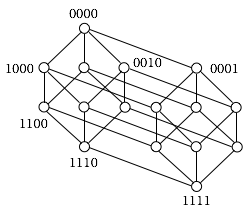
\includegraphics[scale=0.6]{FiguresGraph/Isomorphism1}
       \caption{The hypercube $\q_4$ with a partial vertex-labeling by bit-strings.}
  \label{fig:isomorphism1}
\end{center}
\end{figure}

\begin{figure}[hbt]
\begin{center}
       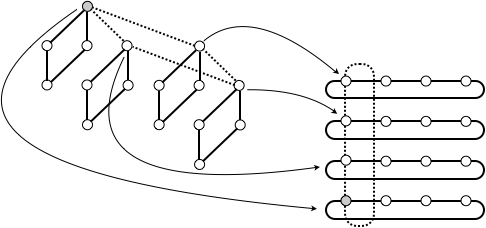
\includegraphics[scale=0.5]{FiguresGraph/Isomorphism2}
       \caption{Transforming $\q_4$ to $\widetilde{\m}_{4,4}$.  The bold edges correspond to horizontal cycles, while the dashed edges correspond to vertical cycles.}
  \label{fig:isomorphism2}
\end{center}
\end{figure}

The isomorphism of Proposition~\ref{prop.graphIsomorphism} is depicted in Figs.~\ref{fig:isomorphism1} and~\ref{fig:isomorphism2}.  We challenge the reader in Exercise~\ref{Exercice:isomorphism} to craft a formal proof of this result, using as a hint the coding scheme (or, bijection) depicted in Fig.~\ref{fig:toruslabel}.
\begin{figure}[hbt]
\begin{center}
       \includegraphics[scale=0.6]{FiguresGraph/toruslabel}
\caption{Hinting at the coding scheme that yields an isomorphism between $\q_4$ and $\widetilde{\m}_{4,4}$.}
  \label{fig:toruslabel}
\end{center}
\end{figure}


\subsection{The {\it de Bruijn} Network $\d_n$}
\label{sec:deBruijn}
\index{de Bruijn network}
\index{de Bruijn graph}

While the family of hypercube networks has few competitors in the world of parallel and distributed computing, in terms of performance and ease of designing algorithms, it does have one major shortcoming that relates to its realizability in hardware.  The basic problem is that each vertex of $\q_n$ has vertex-degree $n$; i.e., hypercubes' vertex-degrees are logarithmic in their numbers of vertices.  This feature makes the hypercube's actual performance much slower than its theoretical performance: each step of a vertex $v$ of $\q_n$ is slowed down by $v$'s having to get inputs from and supply outputs to its $n$ (directed) neighbors.  The phenomenon we are discussing can actually be described {\em geographically}!  The physical area that $\q_n$ occupies grows {\em exponentially} with the common degrees of the network's vertices---because $\q_n$ has $2^n$ vertices which are no more than $n$ edge-traversals from one another.  (This is the ``inverse'' way of talking about logarithmic vertex-degrees.)  In contrast, the space in which we (and our computers) live grows only {\em cubically} with linear distance.  (I.e., we live in $3$-dimensional space!)  The resulting disparity in growth rates means that the wires in large hypercube-connected
computing platforms must inevitably be {\em very} long---in contrast to the unit size of idealized network-edges.  Consequently, electrical signals within a large hypercube must travel long distances in physical space---which means that the physical computer is much slower than its idealized version.  (One finds a more technical discussion of this phenomenon in, e.g., \cite{Ullman84}.)

\smallskip

The just-described shortcoming of hypercubes led researchers for decades (beginning in the 1970s to seek a family of networks whose vertex-degrees stay constant even as one deploys successively larger instances of the network.  We now describe such a family of networks---which combines constant vertex-degrees with logarithmic diameters.  The network family we focus on in this subsection was discovered within the domain of {\it coding theory}---as, coincidentally, was the hypercube.  

\medskip

\index{de Bruijn, Nicolaas Govert} \index{de Bruijn sequence}

In the mid-20-century, Dutch mathematician Nicolaas Govert de Bruijn discovered a way to generate compact sequences that contain all possible strings of a prespecified length.  Focusing on {\em binary} strings---although de Bruijn's strategy works for any finite alphabet---de Bruijn could generate a string of length $2^n +n-1$ which contains every length-$n$ binary string as a substring.  Quite appropriately, such a string is called an order-$n$ {\it de Bruijn sequence}.

It is not obvious that order-$n$ de Bruijn sequences exist for every $n$, but we now plant the
seeds of a proof that they do.  We begin by illustrating two sample sequences in (\ref{eqn:deBruijn-seq}).
\begin{equation}
\label{eqn:deBruijn-seq}
\begin{array}{|l||c|c|}
\hline
n & \mbox{\sc Length-$n$ binary strings}
    & \mbox{\sc Order-$n$ de Bruijn sequence} \\
\hline
\hline
1 &
00, \ 01, \ 10, \ 11  & 00110 \\
\hline
2 &
\begin{array}{l}
000, \ 001, \ 010, \ 011, \\
100, \ 101, \ 110, \ 111 
\end{array}
  & 0001110100 \\
\hline
\end{array}
\end{equation}
The table in (\ref{eqn:deBruijn-seq}) spawns several interesting questions:
\begin{itemize}
\item
Do de Bruijn sequences exist for every $n$?
\item
If so, 
  \begin{itemize}
  \item
How does one compute them?
  \item
Can one always find a de Bruijn sequence of length $2^n +n-1$?
  \item
Can one find de Bruijn sequences of length $< 2^n +n-1$?
  \end{itemize}
%{\Arny (SOME GOOD EXERCISES HERE)} 
\end{itemize}
The answers to all of these questions---and the connection of de Bruijn sequences to the current chapter---reside in the family of directed graphs called {\it de Bruijn graphs} (or, {\it networks}).
(The term used varies by intended application---mainly, coding theory and [the interconnection networks of] parallel computer architectures.  We use the names interchangeably.)
\index{de Bruijn graph} \index{de Bruijn network}
\begin{figure}[hbt]
\begin{center}
       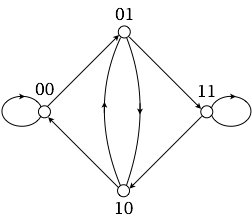
\includegraphics[scale=0.45]{FiguresGraph/dB2by2}
       \caption{The $4$-vertex, order-$2$ de Bruijn network.}
  \label{fig:dB2by2}
\end{center}
\end{figure}

\begin{figure}[hbt]
\begin{center}
       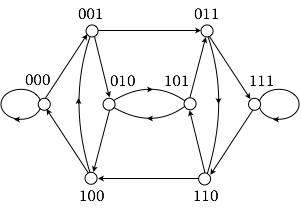
\includegraphics[scale=0.46]{FiguresGraph/dB2by3}
       \caption{The $8$-vertex, order-$3$ de Bruijn network.}
  \label{fig:dB2by3}
\end{center}
\end{figure}

For every integer $n \in \N^+$, the {\it order-$n$ de Bruijn network} is the {\em directed} graph $\d_n$ whose vertices comprise the set of length-$n$ binary strings.\footnote{While {\em binary} de Bruijn networks are the most frequently encountered ones, one can also find de Bruijn networks whose vertices comprise all length-$n$ strings over larger finite alphabets.  Such extended families also find applications in coding theory.}  The sets $\n_{\fd_2}$ and $\n_{\fd_3}$ appear in Table (\ref{eqn:deBruijn-seq}).

\smallskip

$\d_n$ is a regular directed graph; its vertices all have in-degree $2$ and out-degree-$2$.  Each vertex of $\d_n$ is a binary string of length $n \geq 1$; hence it can be written in the form $\beta x$, where $\beta \in \{0, \ 1\}$ is a {\it bit} and $x$ is a length-$(n-1)$ binary string.

\smallskip

The $2^{n+1}$ arcs of $\d_n$ come in pairs specified as follows.  For each $\beta \in \{0,1\}$ and for each length-$(n-1)$ binary string $x$, $\d_n$ has the two arcs
\[ (\beta x \rightarrow x0) \ \ \ \mbox{ and } \ \ \  (\beta x \rightarrow x1) \]
We enumerate $\a_{\fd_3}$ in Table (\ref{eqn:deBruijn-arcs}).
\begin{equation}
\label{eqn:deBruijn-arcs}
{\small
\begin{array}{|ccccc|}
\hline
\mbox{\sc Source vertex} & & \mbox{\sc Target vertex} & & \mbox{\sc Target vertex} \\
\hline \hline
{\displaystyle
\left.
\begin{array}{c}
000 \\
001 \\
010 \\
011 \\
100 \\
101 \\
110 \\
111
\end{array}
\right\}
} &
\mbox{\sc goes to} 
  &
{\displaystyle
\left\{
\begin{array}{c}
000 \\
010 \\
100 \\
110 \\
001 \\
011 \\
101 \\
111
\end{array}
\right.
}
  &
\mbox{\sc and to}
  &
{\displaystyle
\left\{
\begin{array}{c}
001 \\
011 \\
101 \\
111 \\
000 \\
010 \\
100 \\
110
\end{array} 
\right.
}
 \\
\hline
\end{array}
}
\end{equation}

\smallskip

For each $n \in \N^+$, $\d_n$ has diameter $n$.  To see why this is true, note that following any one of $\d_n$'s arcs, say from vertex $x$ to vertex $y$, consists of ``rewriting'' the length-$n$ string $x$ as the length-$n$ string $y$.  The diameter bound therefore follows by showing that, for any two string-vertices of $\d_n$, say vertex $u$ and vertex $v$, one can rewrite $u$ as $v$ by traversing a sequence of arcs---i.e., a directed path---of length at most $n$.  Observe, for instance, that the path in $\d_3$ described schematically as follows
\[ 000 \ \rightarrow \ 001 \ \rightarrow \ 011 \ \rightarrow \ 111 \]
leads vertex $000$ to vertex $111$, by rewriting string $000$ as string $111$.  The diameter bound is now an immediate consequence of the existence in de Bruijn graphs of cycles that contain every vertex precisely once!  We are not yet ready to study these cycles, although we soon will be.

\smallskip

\index{graph!Hamiltonian cycle} \index{Hamiltonian cycle}

A {\it Hamiltonian cycle} in an $n$-vertex graph $\g$ is a length-$n$ cycle that contains every vertex of $\g$ precisely once.  A {\it directed Hamiltonian cycle} in an $n$-vertex digraph $\h$ is a length-$n$ directed cycle that contains every vertex of $\h$ precisely once.  We study Hamiltonian cycles in some detail in Section~\ref{sec:Hamiltonian-cycle}.  And, we prove in Section~\ref{sec:hamiltonian-named-graphs} (see Proposition~\ref{thm:named-graph-Hamiltonian}(e)) that every de Bruijn network is directed-Hamiltonian!

\bigskip

Stepping back from the structural specifics of $\d_n$, we now see that de Bruijn networks provide us with a {\em bounded-degree}---specifically, a degree-$2$---family of networks each of whose constituent digraphs has diameter that is {\em logarithmic} in its size!  In this regard, at least, de Bruijn networks have exactly the same cost-performance as hypercubes---both graphs have $2^n$-vertices and diameter $n$---{\em but the de Bruijn networks achieve this with bounded degrees}.  Even more dramatic:  It has been shown that sophisticated algorithmic techniques can achieve roughly equivalent computational efficiency, on a broad range of significant computational problems, using de Bruijn networks as using like-sized hypercubes \cite{AnnexsteinBR90, BermondP89, Ullman84}.


\ignore{**********

\begin{prop}
\label{thm:deBruijn-Hamiltonian}
For all $n \in \N^+$, $\d_n$ contains a {\em directed Hamiltonian cycle}, 
\index{directed Hamiltonian cycle in a digraph}
i.e., a length-$2^n$ directed cycle of the form
\begin{equation}
\label{eq:deBruijn-cycle}
 x \ \rightarrow \ y_1 \ \rightarrow \ y_2 \ \rightarrow \cdots
\ \rightarrow \ y_{2^n-1} \ \rightarrow \ x
\end{equation}
that contains every vertex of $\d_n$ precisely once; i.e.:
\begin{itemize}
\item
$\{x, \ y_1, \ y_2, \ldots, \ y_{2^n-1}\} \ = \ \n_{\fd_n}$.
\item
All of the ``$y$-vertices'' that appear in cycle
(\ref{eq:deBruijn-cycle}) differ from $x$ and from each other.
\end{itemize}
\end{prop}

The simplest proof of this result has two steps, each of which introduces a topic that we have not 
yet developed.  We develop these concepts plus the proof in 
Appendix~\ref{Appendix:deBruijn-Hamiltonian}.

***********}

%{\Denis Add a word here about hamiltonian and Eulerian and refer to the appendix...}

\ignore{************

\noindent {\bf (1)}
%
For any directed graph $\g$, the {\it line digraph} \index{line graph}
\index{line digraph} of $\g$, denoted $\Lambda(\g)$, is the following
directed graph.
\begin{itemize}
\item
The vertices of $\Lambda(\g)$ are the arcs of $\g$:
\[ \n_{{\Lambda}({\cal G})} \ = \ \a_{\fg} \]
\item
For each pair of arcs of $\g$ of the form
\[ \big[a_{x,y} = (x \ \rightarrow \ y) \big] \ \ \ \mbox{ and } \ \ \ 
\big[a_{y,z} = (y \ \rightarrow \ z) \big]
\]
i.e, arcs such that the endpoint of the first arc is the source of the
second arc, $\Lambda(\g)$ contains an arc $(a_{x,y} \ \rightarrow
\ a_{y,z})$.
\end{itemize}
The relevance of this topic to this section is that the line graph of
every de Bruijn network $\d_n$ is the ``next bigger'' de Bruijn
network, $\d_{n+1}$.  Let us verify this claim.

\begin{prop}
\label{thm:deBruin-linegraph}
For all $n \in \N^+$,
$\d_{n+1}$ is the line digraph of $\d_n$: $\d_{n+1} \ = \ \Lambda(\d_n)$.
\end{prop}

\begin{proof}
Each vertex of $\Lambda(\d_n)$ is an arc of $\d_n$, hence has the form
\[ (\beta x \ \rightarrow \ x \gamma) \]
for $x$ a length-$(n-1)$ binary string and $\beta, \gamma \in
\{0,1\}$.  Let us associate vertex $\beta x \gamma$ of $\d_{n+1}$ with
this vertex of $\Lambda(\d_n)$.

\smallskip

Note first that each arc of $\d_{n+1}$ has the form
\[ (\delta y \varepsilon \ \rightarrow \ y \varepsilon \varphi), \]
where $y$ is a length-$(n-2)$ binary string and $\delta, \varepsilon,
\varphi \in \{0,1\}$.  By our association of vertices of $\d_{n+1}$ with
arcs of $\d_n$, this arc of $\d_{n+1}$ does, indeed, correspond to two
successive arcs of $\d_n$.   The first of these successive arcs
{\em enters} vertex $y \varepsilon$ of $\d_n$; the second {\em leaves}
that vertex.

Note next that, given any two successive arcs of $\d_n$, say
\[
(\rho \sigma z \ \rightarrow \ \sigma z \tau) \ \ \ \mbox { and } \ \ \
(\sigma z \tau \ \rightarrow \  z \tau \xi)
\]
where $z$ is a length-$(n-2)$ binary string and $\rho, \sigma, \tau,
\xi \in \{0,1\}$, there is, indeed, an arc of $\d_{n+1}$ of the form
\[ (\rho \sigma z \tau \ \rightarrow \ \sigma z \tau \xi) \]
This means that the digraph $\d_{n+1}$ is identical to the digraph
$\Lambda(\d_n)$, modulo a renaming of vertices and arcs.\footnote{Technically,
  we are asserting that the digraphs ${\cal D}_{n+1}$ and ${\Lambda}({\cal D}_n)$ 
  are {\it isomorphic} to one another.  The topic of
  graph isomorphism is beyond the scope of this text, but our informal
  description provides all the details one would need to formalize the
  described isomorphism.}

The described correspondence between the vertices and arcs of $\d_{n+1}$
and $\Lambda(\d_n)$ completes the proof.  \qed
\end{proof}

\begin{figure}[hbt]
\begin{center}
       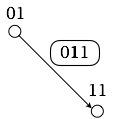
\includegraphics[scale=0.6]{FiguresGraph/dBlabelEdge}
\caption{Illustrating how to label each arc of a de Bruijn network by
  concatenating the labels of the vertices incident to the arc and
  compacting the common intermediate bits.  In the depicted example,
  the vertex-labels $01$ and $11$ combine to yield the arc-label $011$.}
  \label{fig:dBlabelEdge}
\end{center}
\end{figure}

\medskip

\noindent {\bf (2)}
{\it Eulerian cycles (or tours)}. \index{Eulerian cycle}
\index{Eulerian tour} A {\it directed Eulerian cycle} in a digraph
$\g$ is a directed cycle that contains each arc of $\g$ precisely
once.  We will see, later in this chapter, a truly elementary
argument, based on vertex-degrees, which proves that every de Bruijn
digraph has a directed Eulerian cycle.  This demonstration will
combine with Proposition~\ref{thm:deBruin-linegraph} to complete the
proof of Proposition~\ref{thm:deBruijn-Hamiltonian}.  \qed
%\end{proof}
********}

